\title{GitHubを用いた開発フローの判別分析}
\author{プロジェクトマネジメントコース\\
ソフトウェア開発管理グループ\\
矢吹研究室\\
1242132\\
若月 純}
\date{}
\begin{document}
\maketitle
%本テンプレートの余白は,卒論マニュアルで指示されたものとは違っているが,1ページあたりの文字数は40文字x40行と,卒論マニュアル通りになっている.文字間隔や行間隔を調整して,余白をマニュアル通りにすることもできるが,それでは文章が読みにくくなるため,このような対応をしている.

%\noindent
□□□□□□□□□■□□□□□□□□□■□□□□□□□□□■□□□□□□□□□■
□□□□□□□□□■□□□□□□□□□■□□□□□□□□□■□□□□□□□□□■
□□□□□□□□□■□□□□□□□□□■□□□□□□□□□■□□□□□□□□□■
□□□□□□□□□■□□□□□□□□□■□□□□□□□□□■□□□□□□□□□■
□□□□□□□□□■□□□□□□□□□■□□□□□□□□□■□□□□□□□□□■
□□□□□□□□□■□□□□□□□□□■□□□□□□□□□■□□□□□□□□□■
□□□□□□□□□■□□□□□□□□□■□□□□□□□□□■□□□□□□□□□■
□□□□□□□□□■□□□□□□□□□■□□□□□□□□□■□□□□□□□□□■
□□□□□□□□□■□□□□□□□□□■□□□□□□□□□■□□□□□□□□□■
□□□□□□□□□■□□□□□□□□□■□□□□□□□□□■□□□□□□□□□■
□□□□□□□□□■□□□□□□□□□■□□□□□□□□□■□□□□□□□□□■
□□□□□□□□□■□□□□□□□□□■□□□□□□□□□■□□□□□□□□□■
□□□□□□□□□■□□□□□□□□□■□□□□□□□□□■□□□□□□□□□■
□□□□□□□□□■□□□□□□□□□■□□□□□□□□□■□□□□□□□□□■
□□□□□□□□□■□□□□□□□□□■□□□□□□□□□■□□□□□□□□□■
□□□□□□□□□■□□□□□□□□□■□□□□□□□□□■□□□□□□□□□■
□□□□□□□□□■□□□□□□□□□■□□□□□□□□□■□□□□□□□□□■
□□□□□□□□□■□□□□□□□□□■□□□□□□□□□■□□□□□□□□□■
□□□□□□□□□■□□□□□□□□□■□□□□□□□□□■□□□□□□□□□■
□□□□□□□□□■□□□□□□□□□■□□□□□□□□□■□□□□□□□□□■
□□□□□□□□□■□□□□□□□□□■□□□□□□□□□■□□□□□□□□□■
□□□□□□□□□■□□□□□□□□□■□□□□□□□□□■□□□□□□□□□■
□□□□□□□□□■□□□□□□□□□■□□□□□□□□□■□□□□□□□□□■
□□□□□□□□□■□□□□□□□□□■□□□□□□□□□■□□□□□□□□□■
□□□□□□□□□■□□□□□□□□□■□□□□□□□□□■□□□□□□□□□■
□□□□□□□□□■□□□□□□□□□■□□□□□□□□□■□□□□□□□□□■
□□□□□□□□□■□□□□□□□□□■□□□□□□□□□■□□□□□□□□□■
□□□□□□□□□■□□□□□□□□□■□□□□□□□□□■□□□□□□□□□■
□□□□□□□□□■□□□□□□□□□■□□□□□□□□□■□□□□□□□□□■
□□□□□□□□□■□□□□□□□□□■□□□□□□□□□■□□□□□□□□□■
□□□□□□□□□■□□□□□□□□□■□□□□□□□□□■□□□□□□□□□■
□□□□□□□□□■□□□□□□□□□■□□□□□□□□□■□□□□□□□□□■
□□□□□□□□□■□□□□□□□□□■□□□□□□□□□■□□□□□□□□□■
□□□□□□□□□■□□□□□□□□□■□□□□□□□□□■□□□□□□□□□■
□□□□□□□□□■□□□□□□□□□■□□□□□□□□□■□□□□□□□□□■
□□□□□□□□□■□□□□□□□□□■□□□□□□□□□■□□□□□□□□□■
□□□□□□□□□■□□□□□□□□□■□□□□□□□□□■□□□□□□□□□■
□□□□□□□□□■□□□□□□□□□■□□□□□□□□□■□□□□□□□□□■
□□□□□□□□□■□□□□□□□□□■□□□□□□□□□■□□□□□□□□□■
■■■■■■■■■■■■■■■■■■■■■■■■■■■■■■■■■■■■■■■■
□□□□□□□□□■□□□□□□□□□■□□□□□□□□□■□□□□□□□□□■%文字数チェック用

\chapter*{謝辞}

本研究を進めるにあたり,矢吹研究室矢吹太朗准教授には,多くの時間をご指導にさいて頂きました.また,先行研究を行った小野寺航己先輩をはじめ矢吹研究室の皆様には,多くの知識や示唆を頂きました.
協力していただいた皆様に感謝の気持ちと御礼を申し上げます.


\tableofcontents%目次

\chapter{序論}
当研究は,GitHubを用いた開発フローの判別分析を行う.開発フローとは,開発の手順,ルールである.

GitHubを用いた開発フローは13種類ある.それぞれの開発フローには,メリット・デメリットがある.そのため,適切な開発フローを選択できる基準が必要である.


先行研究は,プロジェクトをリスクにより分類していた.そのため,選択基準が定性的になっていた.例を1つあげる.メンバのスキルが高く,大規模なプロジェクトの場合,フローが自動化されているイストフローが選択される\cite{onodera2015}.

そこで当研究は,定量的な選択基準を提供することを目指す.

GitHub上のプロジェクトの性質を調査し,決定木分析を行う.
そうすることで,同一の開発フローを選択しているプロジェクトの共通項を見つけることができる.
共通項を見つけることで,開発フローを選択する基準を割り出せると考える.




\chapter{背景}

ソフトウェア開発では,複数のメンバが同時に開発する場合がある.そのため,様々な問題が発生する.課題をチーム間で適切に共有できず,進捗が見えにくくなったり,複数の人たちで1つの製品のソースコードを編集するため,開発内容が競合したりすることもあります.さらに複数の人たちが関わることによって,コードの質を均一化することも難しくなりますし,製品のコードの全容を把握することも難しくなります\cite{ikeda2014}.

このような問題を解決するため,バージョン管理システムを用いる.バージョン管理システムとは,変更履歴を管理するシステムのことである.

バージョン管理システムの種類とトレンドを次に記述する.
\section{バージョン管理システム}

バージョン管理システムには,CVS,Apache Subversion,Git等がある.Apache Subversionは,以下subversionと記述する.

CVSとは,Concurrent Versions Systemの略称で,並行バージョン管理システムを意味します.1990年に開発された比較的歴史の古いバージョン管理ツールです.こちらは集中型のバージョン管理システムになります\cite{matsuda2015}.

Apache Subversionとは,多くの開発現場で使われていたCVSの問題点を改善するために作られたツールです.2000年に開発され,操作がCVSと似ていることから,CVSからSubversionに乗り換えるユーザが多くいました.CVSと同じく集中型バージョン管理システムです\cite{matsuda2015}.

Gitとは,2005年に開発された分散型のバージョン管理ツールです.Linuxカーネルのソースコード管理のために開発されたもので,今では多くの開発者に使われている人気のバージョン管理ツールです\cite{matsuda2015}.


図\ref{worldTrend}と図\ref{japanTrend}は,GoogleTrendを用いて描かれたものである.それぞれの検索の割合を示している.

図\ref{worldTrend}と図\ref{japanTrend}は,2004年1月4日から2016年1月23日まで,コンピュータ,電化製品,を対象としている.
図\ref{worldTrend}は,すべての世界を対象としている.
図\ref{japanTrend}は,日本のみを対象としている.

\begin{figure}[H]
\centering 
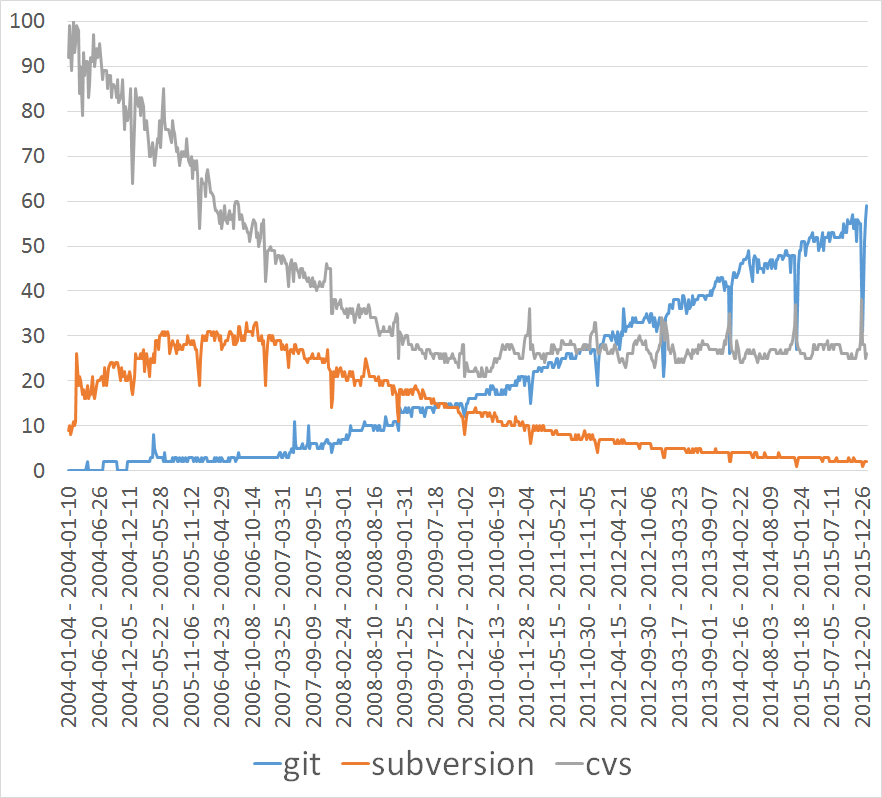
\includegraphics[width=13cm]{worldTrend.png}
\caption{世界でのバージョン管理システムのトレンド}\label{worldTrend}
\end{figure}
図\ref{worldTrend}より,世界では,最もGitがトレンドになっていることがわかる.
2004年はCVSが最も人気が高かった.しかし,subversionの台頭により,2004年以降人気が落ちていっていることがわかる.

Gitが台頭してきたのは,2005年ごろである.このころから,人気は上昇を続ける一方である.
2009年に,Gitは,subversionの人気を超えた.
2011年に,Gitは,CVSの人気を超えた.

こうして,2015年は,最もGitが人気になっている.

\begin{figure}[H]
\centering 
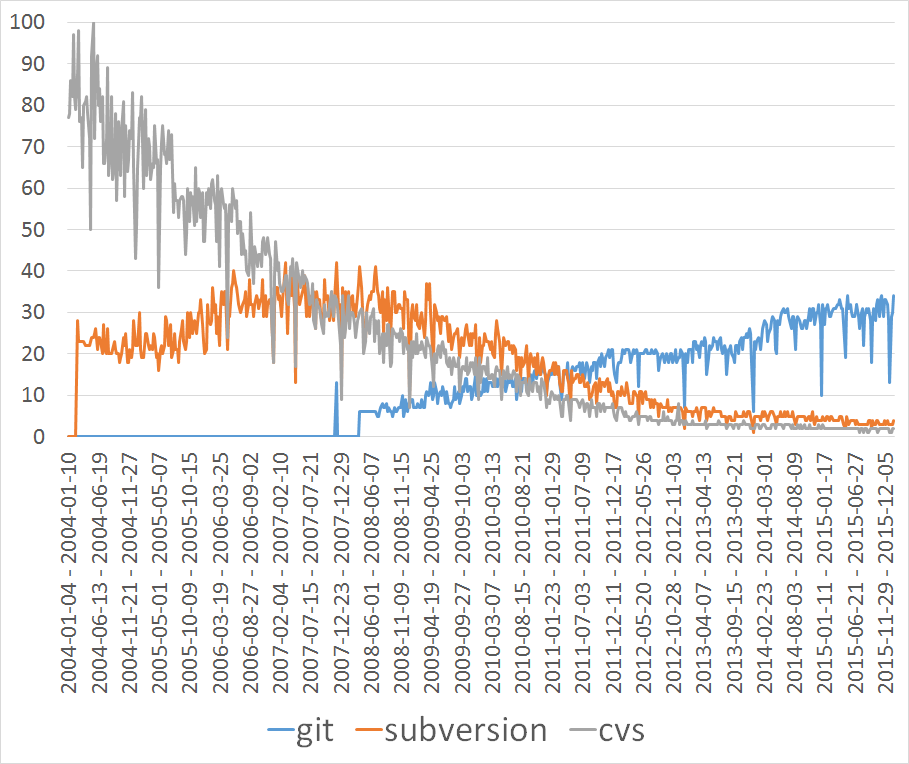
\includegraphics[width=13cm]{japanTrend.png}
\caption{日本でのバージョン管理システムのトレンド}\label{japanTrend}
\end{figure}
図\ref{japanTrend}より,日本でも,最もGitがトレンドになっていることがわかる.
2004年はCVSが最も人気が高かった.しかし,subversionの台頭により,2004年以降人気が落ちていっていることがわかる.

Gitが台頭してきたのは,2008年ごろである.このころから,人気は上昇を続ける一方である.
2010年に,Gitは,CVSの人気を超えた.
2011年に,Gitは,subversionの人気を超えた.

こうして,2015年は,最もGitが人気になっている.

この世界と日本の状況を踏まえ,バージョン管理システムのトレンドについて考察する.

まず,世界と日本の状況を比較する.

図\ref{worldTrend}と図\ref{japanTrend}の技術が伸びを見せる年式に注目する.
世界では,Gitが2005年に台頭してきた.しかし,日本ではGitが台頭してきたのは2008年からである.

ここから,日本に新しい技術が入ってくるのは,世界よりも遅いことが言える.
これは,日本が海外から新しい技術を輸入しているためだと考えられる.
海外の技術は,その土地の言葉で書かれている.そのため,翻訳する必要があるので,技術を輸入し,定着するまでに3年かかっている.


また,日本独自の開発手順があることが言える.
世界のトレンドでは,Git,CVS,subversionの順である.
しかし,日本のトレンドでは,Git,subversion,CVSの順である.

以上の調査により,最も人気があるバージョン開発システムは,Gitであることがわかった.

そのため,本研究では,バージョン管理システムのGitを提供するサービスのGitHubを用いる.
GitHubについての詳しい説明を,次に記述する.

\section{GitHub}

GitHubとは,Gitリポジトリのホスティング機能をもつ.また,スローガンにSocialCodingをかかげているように,複数人で共同開発を行いやすくするための機能を提供している.機能とは,トラッキングや管理を行うためのIssue,ソースコードの差分を論議するためのPull Request等がある.

GitHubは2008年のサービス開始以来,年率100%という成長率で登録ユーザー数やレポジトリ数を伸ばしてきて,オープンソースの世界ではデファクトのプラットフォームとなっている.2015年6月現在,GitHubの登録ユーザー数は970万,レポジトリ数は2330万.最近ではMicrosoftやOracleといったトラディショナルなIT企業もGitHubにレポジトリを用意するようになってきているし,広く知られたメジャーなオープンソース製品の多くがGitHubをプロジェクトのホスト先に選ぶのがここ数年のトレンドだ\cite{Nishimura2015}.

主な具体例として,アップルがSwiftのOSS化をGitHubで行った事例がある.
Appleは,iOSやOS Xの開発言語として提供してきたプログラミング言語のSwiftをオープンソースとして公開した.今回オープンソース化されたのは,ソースコードを実行形式に変換するコンパイラと,プログラムの基本機能をまとめた標準ライブラリなどである.従来は,iOS/OS X向けのソフトウェアしか開発できなかったが,Linuxへの移植版も公開している.
そして,AppleがSwiftを公開した場所もGitHubであった.
Chacon氏は,今回のSwiftのオープンソース化の特徴として,コミュニティーとの連携を強調した.Swiftに対するプルリクエストがすでに社外から500件以上も寄せられており,そのうち349件が統合済みだという.中には,誤字の指摘なども含まれるが,Appleの開発ツール部門のシニアディレクターで,Swiftの主要な開発者であるChris Lattner氏が「小さな改善でも,多くの人が参加するきっかけになる」とツイートしていると紹介した\cite{kachi2015}.


日本でも,セミナーや,行政活動にGitHubを用いる等,盛り上がりをみせている.
具体例として,和歌山県が自治体として最初にGitHub公式アカウントを取得した例をあげる.
和歌山県は自治体としては初めて公共アカウントを取得し,ウェブサイトで公開した情報をGitHubでも公開するなど実際に活用を進めている.今回の訪問は和歌山県庁での活用に注目しているというGitHub側が,現場の話を直接知り,今後の支援につなげたいとの要望から実現したもので,知事との対談に先駆けて,庁内のオープンデータ化を担当する職員や活動を支援する関係者らとも意見を交換した\cite{nonoshita2015-1}.

また,初心者向けのイベントが豊富なことも,人気の一つである.
初心者から参加できるGitHub習得イベント「GitHub Patchwork」が神戸で開催された.
GitHub Patchworkは,GitHubを基礎から学べるオンライン教材「Git-it」をみんなで一緒に学ぶというイベント.2年前にサンフランシスコのGitHub本社で実施されたのをきっかけに世界各地で開催されるようになり,現在14カ国で44件のイベントが実施されている.
参加者からは「以前からGitHubに興味があったが,なかなか勉強する機会がなかったため,今回の参加をきっかけに活用したい」という声が多く聞かれた\cite{nonoshita2015-2}.

しかし,盛り上がりをみせているGitHubにも,問題点はある.
GitHubでホスティングされたプロジェクトで作業する開発者が,自分たちが「無視され」,サポートが得られないとの苦情を公開書簡にて表明している.
この公開書簡はGitHubのWebサイトの管理とサポートチャネルへの不満を綴ったもので,1000人以上の開発者が賛同している.
書簡では,「もしGitHubそのものがオープンソースだったら,われわれはコミュニティーとしてこれらの機能を実装する.われわれはこういうことを得意としているんだ!」と記している.
GitHubの代表者は米ZDNetに対し,「オープンソースはGitHubにとって極めて重要で,今回のフィードバックを真剣に受け止めている.議論されたイニシアティブの幾つかに取り組んでおり,オープンソースのメンテナーたちと積極的な関係を持ち,彼らのコミュニティーにとってGitHubが素晴らしい体験となるようにしたい」と語った\cite{Charlie2016}.

ここまで,GitHubが注目を受けている背景について紹介した.
様々なコミュニティがGitHubを使っている.

GitHub特有の開発を補助する機能が多い.機能を一部抜粋して,説明を記述する.



\section{GitHub用語}

\subsection{リポジトリ}

ファイルやディレクトリの状態を記録する場所.

\subsection{リモートリポジトリ}

手元に置いてあるローカルなリポジトリ以外の,ネット上に置かれたリポジトリのこと.

\subsection{commit}

ファイルやディレクトリの変更をリポジトリに記録する機能である.


\subsection{clone}

ネット上にあるリポジトリをローカルにコピーする機能である.


\subsection{Origin}

clone元のリモートリポジトリのこと.


\subsection{Push}

リモートリポジトリに自分の変更履歴がアップロードされ,リモートリポジトリ内の変更履歴がローカルリポジトリの変更履歴と同じ状態にする機能である.


\subsection{branch}

履歴の流れを分岐して記録していくためのもの.分岐したブランチは,他のブランチの影響を受けないため,同じリポジトリ中で複数の変更を同時に進めていける機能である.


\subsection{pull}

リモートリポジトリから最新の変更履歴をダウンロードしてきて,自分のローカルリポジトリにその内容を取り込む機能である.


\subsection{Pull Request}

相手に対して自分の変更ををpullしてもらうように要求する機能である.


\subsection{Revert}

ステージングエリアに追加した変更を取り消す機能である.

\subsection{タグ}

コミットを参照しやすくするために,わかりやすい名前を付ける機能である.


\subsection{Label}

自由に作成でき,Issueをフィルタリングできる機能である.


\subsection{Merge}

当該ブランチに対して別のブランチの差分を取り込むことである.


\subsection{Fork}

GitHubのサービスで,相手のリポジトリを自分のリポジトリとしてコピー・保持できる機能ある.


\subsection{Issue}

ソフトウェア開発におけるバグや議論などをトラッキングして管理するために発行する.

\subsection{デプロイ}

ソフトウェアの分野で,開発したソフトウェアを利用できるように実際の運用環境に展開する.


\subsection{リリース}

プロセスを次の段階に進めることを認める機能である.


\subsection{Watch}

リポジトリに関する情報をNotificationsに表示する機能である.

\subsection{Star}

リスト一覧からリポジトリを探すことが出来るようにする機能である.
また,注目度を表す指標にもなる.

\subsection{Fork}

GitHub側にある特定のリポジトリを自分のアカウント以下のリポジトリに複製する機能である.

\subsection{人数}
開発人数のことである.
ここでは,Originリポジトリにコミットした人数のことを示す.

\subsection{MileStone}

やるべきタスクの管理にIssueを用いることができるようにする機能である.

\subsection{Wiki}

簡単な記法によってドキュメントを作成,編集するための機能である.






\section{GitHubを用いた開発フロー}
GitHubを使用する手順を開発フローと呼ぶ.開発フローを網羅的に調査した先行研究がある.
先行研究で調査され,本研究で用いた開発フローと,選択基準を以下に記述する.

\subsection{GitHubフロー}

\begin{figure}[H]
\centering 
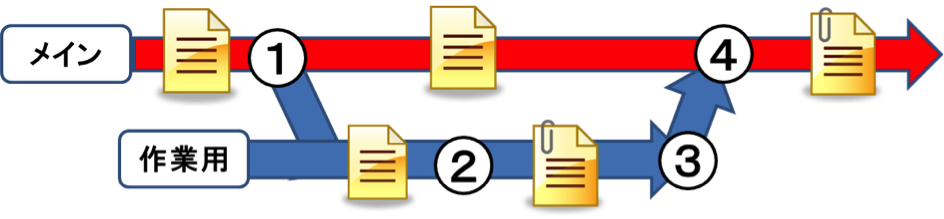
\includegraphics[width=13cm]{github.png}
\caption{GitHubフロー図 出典:\cite{onodera2015}p17}\label{tab:githubフロー}
\end{figure}
\begin{figure}[H]
\centering 
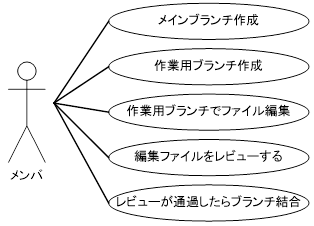
\includegraphics{githubyou.png}
\caption{GitHubフローユースケース図 出典:\cite{onodera2015}p18}\label{tab:githubyou}
\end{figure}
\begin{figure}[H]
\centering 
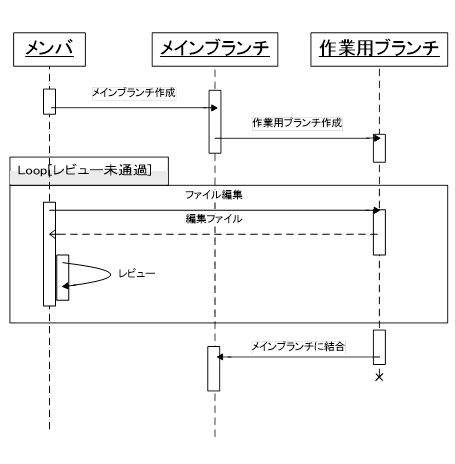
\includegraphics{githubsi.png}
\caption{GitHubフローシーケンス図 出典:\cite{onodera2015}p18}\label{tab:githubsi}
\end{figure}


GitHubフローはGitHub社が実践しているシンプルなワークフローである.
基本的には特定の作業をするブランチを作成するだけなので,作業を始めてデプロイするまでの過程がとてもシンプルです.これはワークフローを実施するまでの学習コストを抑えられるという利点があります.さらに大きな利点として,シンプルであるからこと,多くの開発者がすばやく行うことを可能にします.そして,小さな変更などにも柔軟に対処できるようになります\cite{ohtsuka2014}.


\subsection{Gitフロー}

\begin{figure}[H]
\centering 
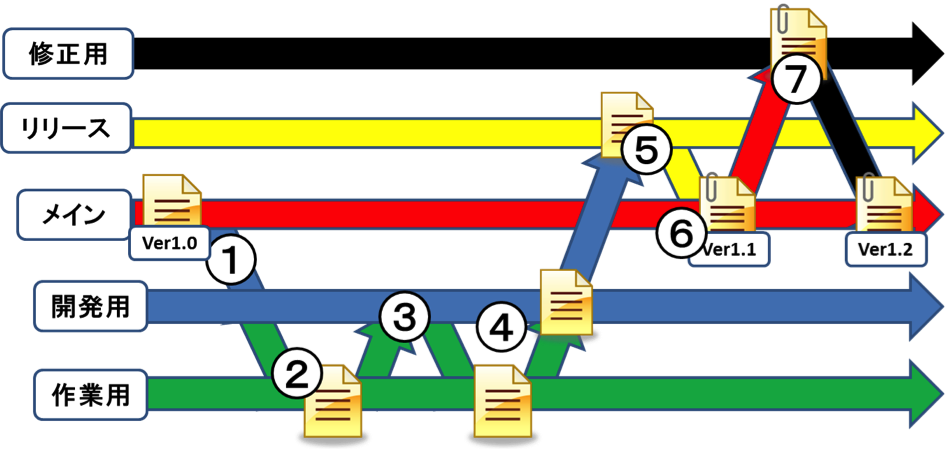
\includegraphics[width=13cm]{git.png}
\caption{Gitフロー図 出典:\cite{onodera2015}p20}\label{tab:gitフロー}
\end{figure}
\begin{figure}[H]
\centering 
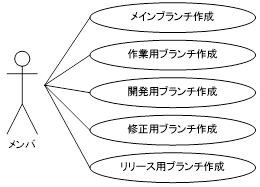
\includegraphics{gityou.png}
\caption{Gitフローユースケース図 出典:\cite{onodera2015}p20}\label{tab:gityou}
\end{figure}
\begin{figure}[H]
\centering 
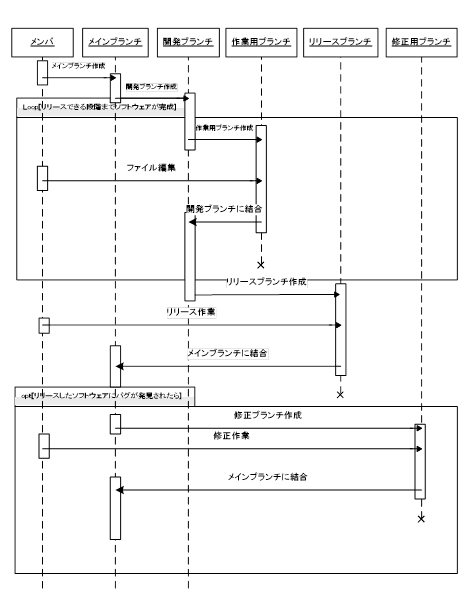
\includegraphics{gitsi.png}
\caption{Gitフローシーケンス図 出典:\cite{onodera2015}p20}\label{tab:gitsi}
\end{figure}

Gitフローはリリース中心の開発スタイルである.
この開発フローは,それぞれのブランチがコードの状態を表している.ソフトウェアのリリースを管理するリリースマネージャーなどが存在し,リリースを中心としたソフトウェア開発に向いている.
しかし,覚えるブランチの状態が多く,開発フロー全体を事前に学習する必要がある.
そのため,gitフローなどのツールのサポートを受けることにより,強制的にフローからはずれない工夫が必要である\cite{ohtsuka2014}.


\subsection{GitLabフロー}


GitLabフローは,GitHubフローをベースにしている.


特徴は,branchにstable branchを採用している点である.
GitLab branchとは,安定状態のbranchを作ることにより,バグが新たに入り込むリスクを減らす効果がある.
GitLab branchは,できるだけ最新のmasterブランチから分岐することで,バグを新たに入り込むリスクを減らせる\cite{Nishimura2015}.



\subsection{日本CAW フロー}

\begin{figure}[H]
\centering 
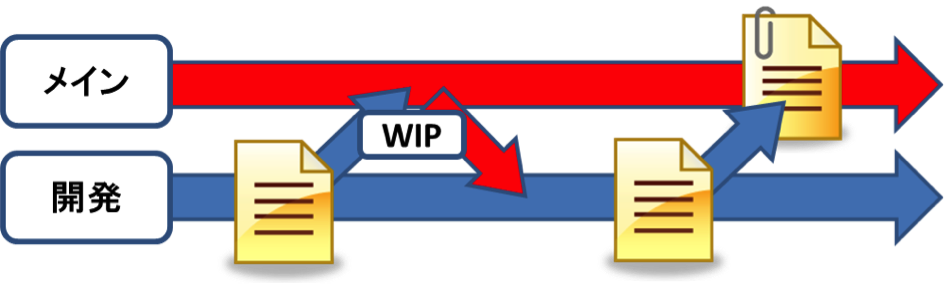
\includegraphics[width=13cm]{nihonCAW.png}
\caption{日本CAWフロー図 出典:\cite{onodera2015}p23}\label{tab:日本CAW}
\end{figure}
\begin{figure}[H]
\centering 
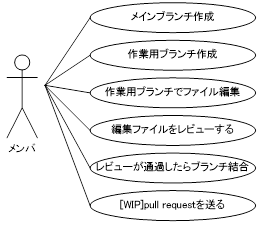
\includegraphics{cawyou.png}
\caption{日本CAWフローユースケース図 出典:\cite{onodera2015}p24}\label{tab:cawyou}
\end{figure}
\begin{figure}[H]
\centering 
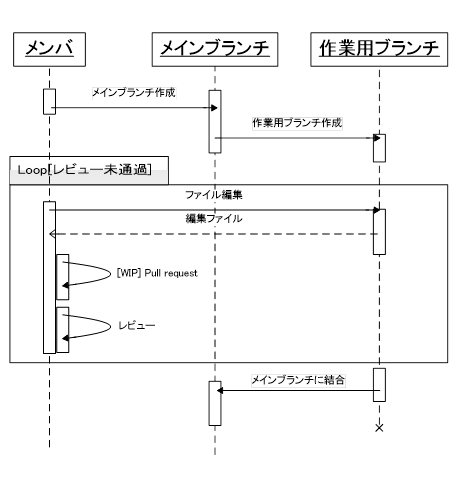
\includegraphics{cawsi.png}
\caption{日本CAWフローシーケンス図 出典:\cite{onodera2015}p24}\label{tab:cawsi}
\end{figure}


日本CAWフローは,日本CAW株式会社が採用しているフローである.
このフローは,GitHub フローをベースにしてPull Requestを活用したスタイルを採用している.
特徴は,WIP PRを採用している点である.
WIP PR(Work In Progress Pull Request)とは,実装の仕方や,コードの設計など,コードに紐づく議論をしやすくするために用いられる.Pull Request作成時に頭に[WiP]を入れる.[WIP]がついたPull Requestはマージされず,議論や確認のために参照される.作成者は議論や確認が済んだらCloseする,といったフローである\cite{harada2014}.




\subsection{LINE フロー}

\begin{figure}[H]
\centering 
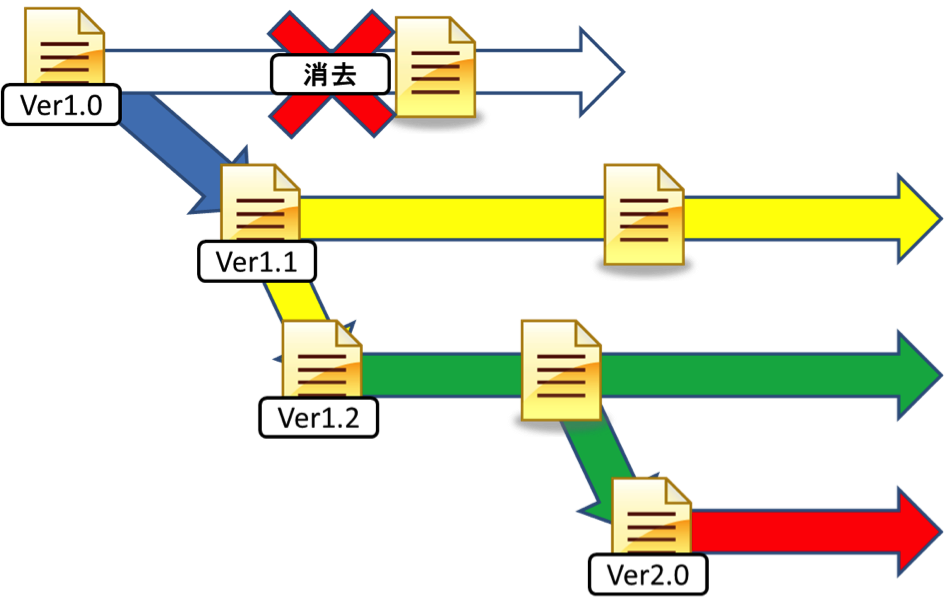
\includegraphics[width=13cm]{LINE.png}
\caption{LINEフロー図 出典:\cite{onodera2015}p31}\label{tab:LINE フロー}
\end{figure}
\begin{figure}[H]
\centering 
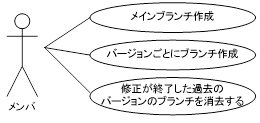
\includegraphics{lineyou.png}
\caption{LINEフローユースケース図 出典:\cite{onodera2015}p32}\label{tab:lineyou}
\end{figure}
\begin{figure}[H]
\centering 
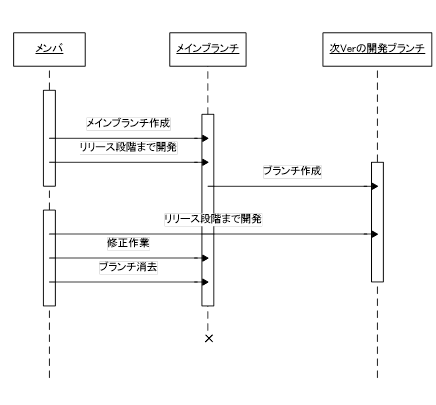
\includegraphics{linesi.png}
\caption{LINEフローシーケンス図 出典:\cite{onodera2015}p32}\label{tab:linesi}
\end{figure}


LINEフローはPull Requestなどを活用して行われる開発フローである.
常にdeploy可能なバージョン毎のmasterを持っているよいう形で運用している.
それぞれがリリース可能なブランチで,開発状況によっては下位のバージョンのコミットが上位のバージョンのコミットより新しい場合がある.
LINEのIOSアプリではバージョン毎に提供する機能や修正を決めていて,QA対象の切り分けがしやすいなどのメリットもあり,1つのmasterにcommitを繋げいく形では運用していない.
現在開発中の最も下位のバージョンの修正がリリースされたら,そのブランチを上位のブランチにマージして下位のブランチを消していく流れで行われる\cite{hayaishi2014}.


\section{GitHubを用いた開発フローの選択基準}
それぞれ異なったリスクがあるため,最適な開発フローを選択する基準をリスクの面から分類された.研究の結果が表\ref{tab:onodera}である.プロジェクトの特徴から最適な開発フローが選択できるようになった.

\begin{table}[H]
 \begin{center}
 \caption{プロジェクトと開発フロー出典:\cite{onodera2015}p62}
  \begin{tabular}{|c|c|c|c|} \hline
    プロジェクトの特徴 & 開発フローの特徴 & 該当する開発フロー \\ \hline
    \shortstack{メンバのスキルが高い \\ 大規模なプロジェクト} & フローが自動化されている & \shortstack{フィヨルドフロー\\イストフロー}\\ \hline
    参加メンバが多い & 複数のリポジトリを使用する & \shortstack{Amingフロー \\ サイボウズフロー \\ 矢吹研フロー\UTF{2460} \\ 矢吹研フロー\UTF{2461}}\\ \hline
    アジャイル型のソフトウェア開発 & \shortstack{アジャイル開発のような \\ 流れが可能} &\shortstack{ Gitフロー \\ キャスレーフロー}\\ \hline
    \shortstack{GitHubを今まで導入した経験が無い \\ プロジェクト} & 使用するブランチが少ない & \shortstack{GitHubフロー \\ 日本CAWフロー \\ はてなブログフロー} \\ \hline
    ソフトウェアに何を盛り込むのかが明確 & 使用済みブランチを破棄 & \shortstack{ラクスルフロー \\ LINEフロー}\\ \hline
  \end{tabular}
  \label{tab:onodera}
  \end{center}
\end{table}


しかし,メンバのスキルが高い,大規模なプロジェクト等,定性的な表現が多い.

そこで当研究では,選択する基準を定量的に分けられるようにすることを目指す.具体例を二つあげる.開発人数が5人の場合かつ,言語がRubyの場合は,GitHubフローが最適である.開発人数が15人の場合かつ,言語がJavaの場合は,Gitフローが最適である,

そうすることで,既存の基準より,適切な開発フローを選択できるようになると考える.








\chapter{目的}


GitHubを用いたソフトウェア開発プロジェクトの性質において,適切な開発フローを選択できるようにするための基準を提供する.








\chapter{手法}
調査準備,調査対象,調査方法,分析準備,分析方法について記述する.

環境は,2種類用いた.
一つ目は,OS X Yosemite バージョン15.15.5である.
二つ目は,Ubuntuである.

\section{調査準備}
調査は,GitHubAPIを用いる.
そのため,GitHubAPIの準備について,記述する.

ここで行う準備の環境は,Ubuntuを想定している.
\subsubsection{curlのインストール}
{
\small
\begin{verbatim}
sudo apt-get install curl
\end{verbatim}
}
\subsubsection{ログイン情報入力を省略}
{
\small
\begin{verbatim}
echo 'ユーザ名:パスワード' > github.passwd
chmod 600 github.passwd
\end{verbatim}
}
\subsubsection{PythonとHTTPアクセスのためのrequestsのインストール}
{
\small
\begin{verbatim}
sudo apt-get install python python-setuptools
sudo easy_install requests
\end{verbatim}
}


\subsubsection{api.pyのダウンロード}
{
\small
\begin{verbatim}
curl -s -u $(cat github.passwd) 
https://raw.githubusercontent.com/taroyabuki/yabukilab/master/library/github/api.py
 > api.py
\end{verbatim}
}
\subsubsection{api.pyについて}
{
\small
\begin{verbatim}
#!/usr/bin/python
# coding: UTF-8

import sys, json, requests

#GitHubのログイン情報をファイルから取得する
#TODO:パスワードに「:」を使っているとダメ
tmp = open('github.passwd').readline().rstrip('\n').split(':');
username = tmp[0]
password = tmp[1]
#print >> sys.stderr, username,password

#APIのURLはコマンドライン引数で与える
url = sys.argv[1]

count = 0
while (url is not None):
  print >> sys.stderr, url
  r = requests.get(url, auth=(username, password))
  print >> sys.stderr, r.headers['status'],
  items = r.json()['items'] if 'items' in r.json() else r.json()
  for item in items:
      count = count + 1
      print json.dumps(item)
  if (r.links.has_key('next')):
    url = r.links['next']['url']
  else:
    url = None
  print >> sys.stderr, count, 'items'
\end{verbatim}
}


\section{調査対象}

調査対象プロジェクトと調査対象指標を記述する.

\subsection{調査対象プロジェクト}

調査するユーザ名とプロジェクト名を記載する.
\begin{table}[H]
 \begin{center}
 \caption{調査対象プロジェクト}
  \begin{tabular}{|l|c|r||r|} \hline
    ユーザ名 & リポジトリ名\\ \hline
    zedapp & zed\\ \hline
    LearnBoost & stylus\\ \hline
    spine & spine\\ \hline
    sirjuddington & SLADE\\ \hline
    sass & sass\\ \hline
    Polymer & polymer\\ \hline
    play & play\\ \hline
    ossec & ossec-hids\\ \hline
    NTU-CCSP & ntu-ccsp.github.io\\ \hline
    neovim & neovim\\ \hline
    aol & moloch\\ \hline
    rackerlabs & mimic\\ \hline
    melonjs & melonJS\\ \hline
    nasa & mct\\ \hline
    waysome & libreset\\ \hline
    knockout & knockout\\ \hline
    KnpLabs & FriendlyContexts\\ \hline
    freifunkMUC & freifunkmuc.github.io\\ \hline
    admc & flex-pilot-x\\ \hline
    dfm & emcee\\ \hline
    adamhjk & dynect\_rest\\ \hline
    ashesi-SE & datasaver\\ \hline
    pyca & cryptography\\ \hline
    karpathy & convnetjs\\ \hline
    tlycken & Contour.jl\\ \hline
    ellisonleao & clumsy-bird\\ \hline
    mozbrick & brick\\ \hline
    tyoshii & bms\\ \hline
    sampsyo & beets\\ \hline
    openstf & adbkit\\ \hline
    CyberAgent & android-gpuimage\\ \hline
  \end{tabular}
  \label{tab:project}
  \end{center}
\end{table}


\subsection{調査対象指標}
調査する指標は,Watch数,Star数,Fork数,commit数,branch数,Release数,人数,言語,行数,ファイル数,バイト数,OpenIssues数,ClosedIssues数,Issues数,OpenPull Request数,ClosedPull Request数,Pull Request数,Label数,OpenMileStone数,ClosedMileStone数,MileStone数,Wiki数,言語,日数,開発フローである.




\section{調査方法}
\subsection{Watch数,Star数,Fork数,commit数,branch数,Release数,人数の調査}
調査は,手動で行う.


\begin{figure}[H]
\centering 
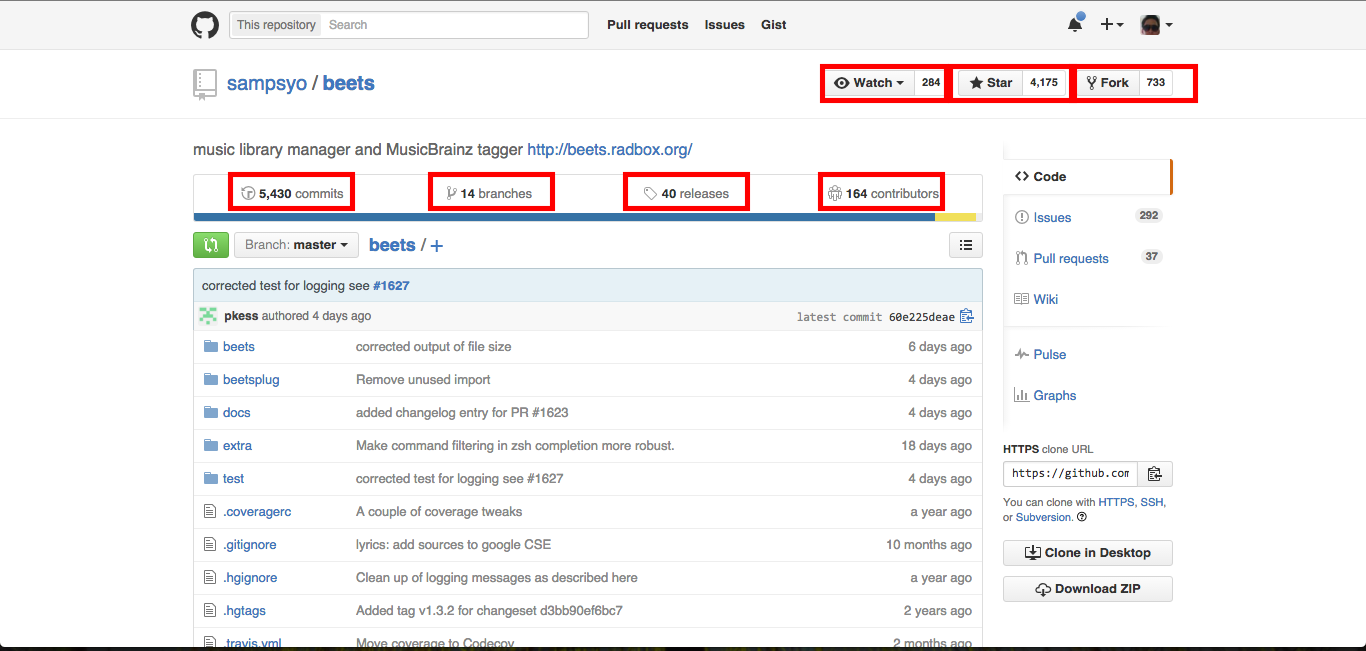
\includegraphics[width=13cm]{Watch.png}
\caption{Watch数,Star数,Fork数,commit数,branch数,Release数,人数の調査}\label{tab:Watch}
\end{figure}
図\ref{tab:Watch}はWatch数,Star数,Fork数,commit数,branch数,Release数,人数の調査画面である.
commitsがcommit数,branchesがbranch数,releasesがRelease数,contributorsが人数である.
赤枠に囲まれている数値を取得する.所得した数値は,"データ一覧.csv"に保存する.



\subsection{言語の調査}
調査は,手動で行う.
\begin{figure}[H]
\centering 
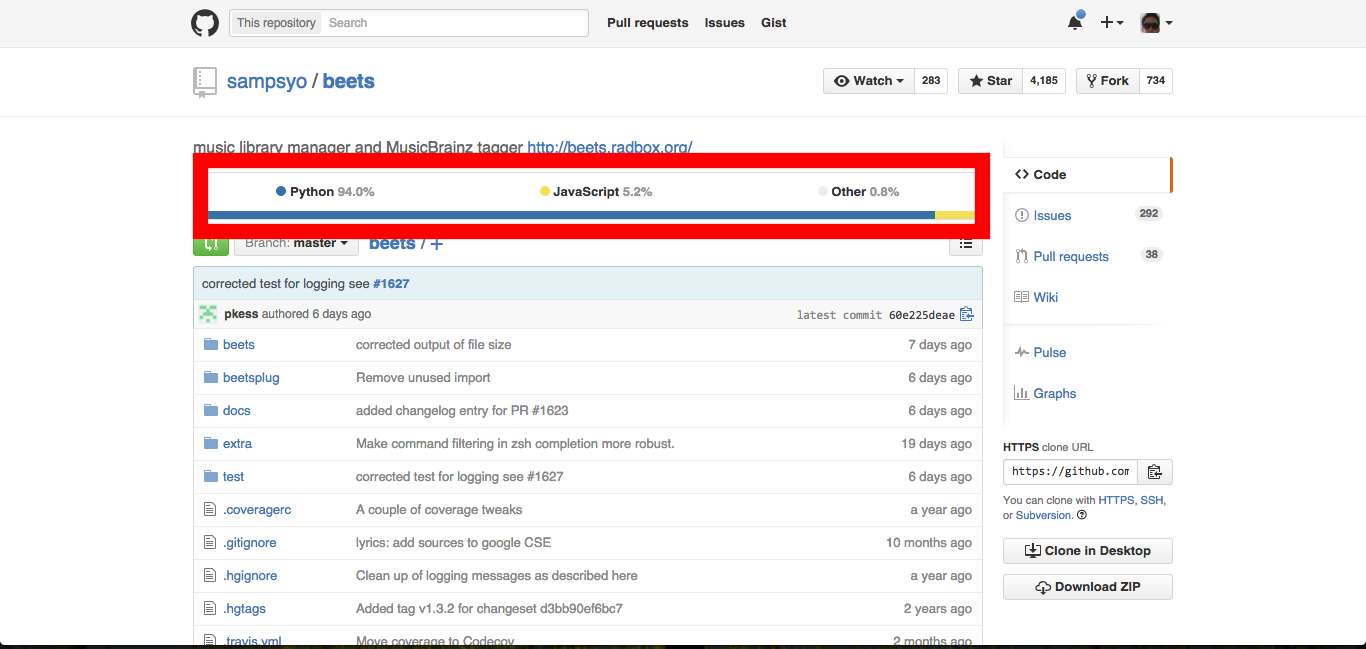
\includegraphics[width=13cm]{language.png}
\caption{言語の調査}\label{tab:言語}
\end{figure}
図\ref{tab:言語}は言語の調査画面である.
赤枠に囲まれている数値を取得する.所得した数値は,"データ一覧.csv"に保存する.


\subsection{OpenIssues数,ClosedIssues数,Issue数の調査}

調査は,手動で行う.

\begin{figure}[H]
\centering 
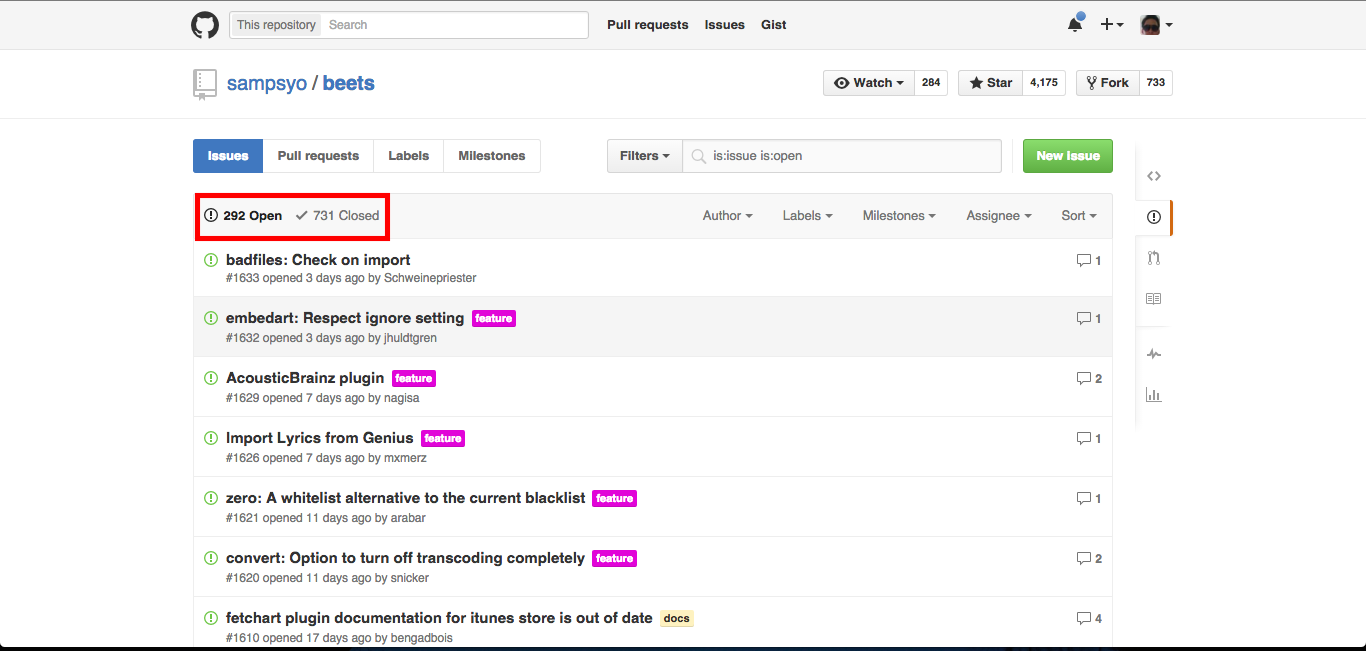
\includegraphics[width=13cm]{Issues.png}
\caption{Issues数の調査}\label{tab:Issues}
\end{figure}
図\ref{tab:Issues}はOpenIssues数,ClosedIssues数,Issue数の調査画面である.OpenがOpenIssues数,ClosedがClosedIssues数である.OpenとClosedの合計がIssue数である.
赤枠に囲まれている数値を取得する.所得した数値は,"データ一覧.csv"に保存する.

\subsection{OpenPull Request数,ClosedPull Request数}
調査は,手動で行う.

\begin{figure}[H]
\centering 
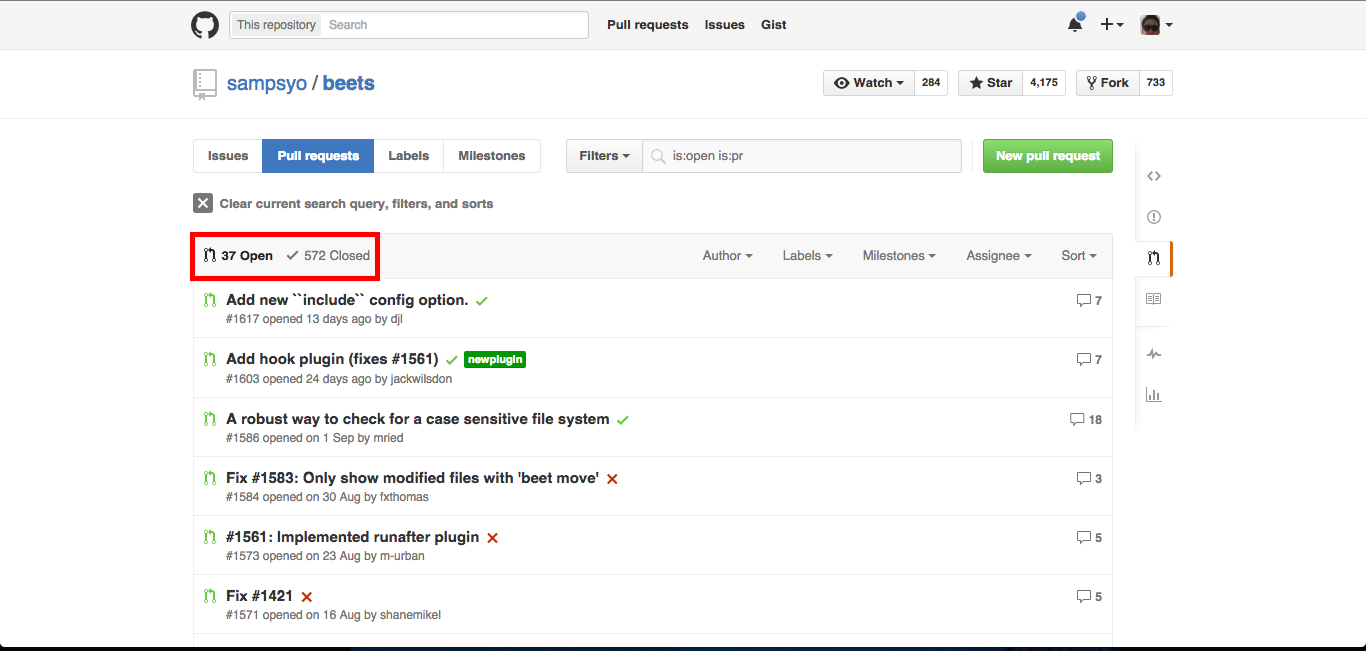
\includegraphics[width=13cm]{PullRequest.png}
\caption{Pull Request数の調査}\label{tab:PullRequest}
\end{figure}

図\ref{tab:PullRequest}はOpenPull Request数,ClosedPull Request数の調査画面である.OpenがOpenPull Request数,ClosedがClosedPull Request数である.OpenとClosedの合計がPull Request数である.
赤枠に囲まれている数値を取得する.所得した数値は,"データ一覧.csv"に保存する.

\subsection{Label数}
調査は,手動で行う.

\begin{figure}[H]
\centering 
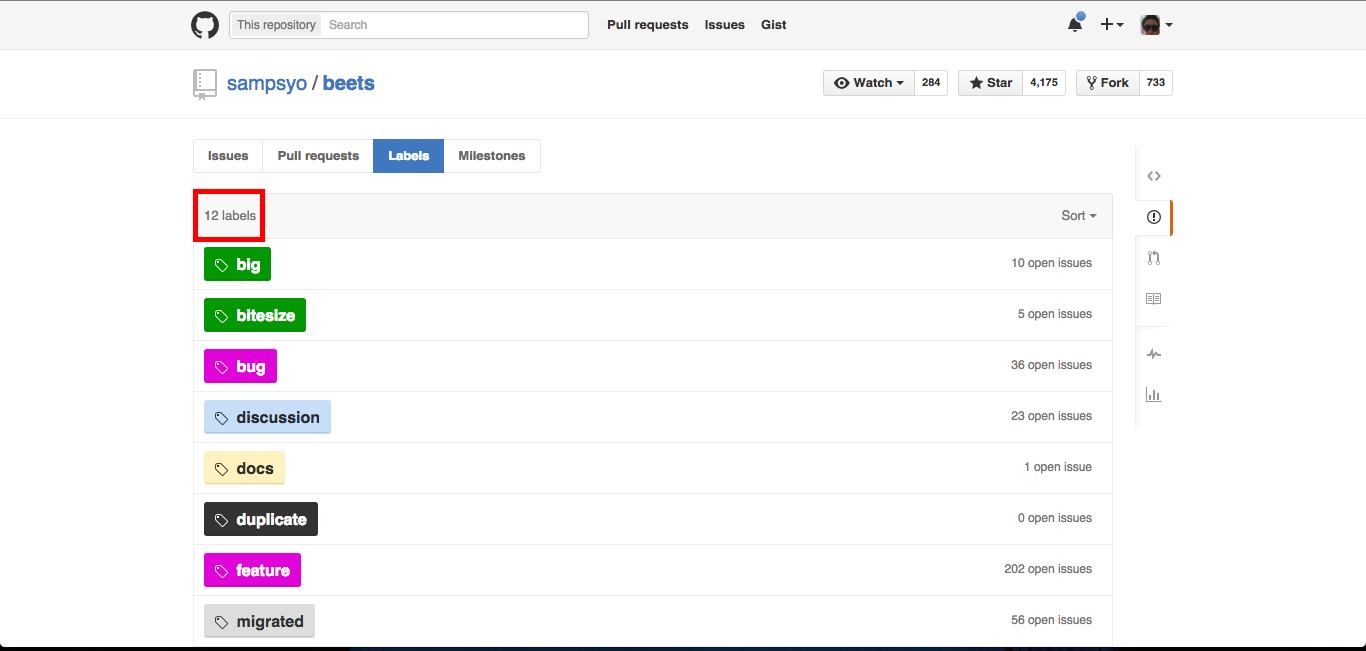
\includegraphics[width=13cm]{Label.png}
\caption{Label数の調査}\label{tab:Label}
\end{figure}

図\ref{tab:Label}はLabel数の調査画面である.labelsがLabel数である.
赤枠に囲まれている数値を取得する.所得した数値は,"データ一覧.csv"に保存する.


\subsection{OpenMilestone数,ClosedMilestone数,Milestone数}
調査は,手動で行う.



\begin{figure}[H]
\centering 
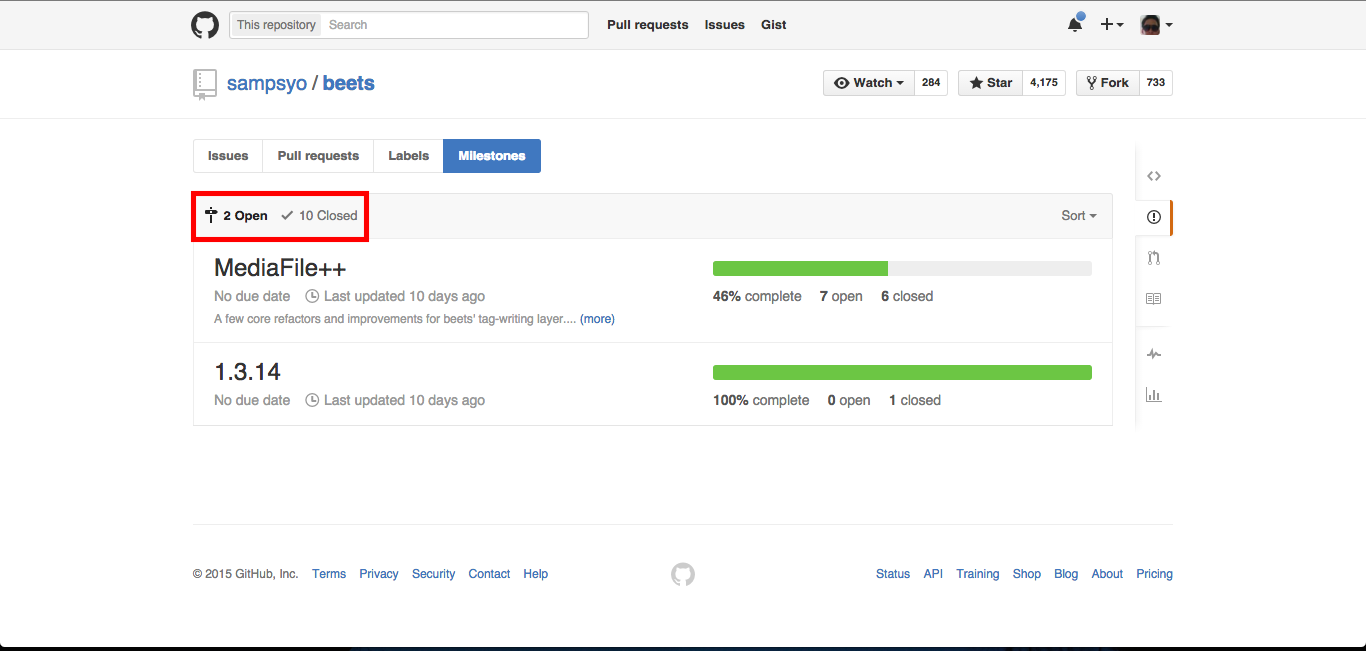
\includegraphics[width=13cm]{Milestone.png}
\caption{Milestone数の調査}\label{tab:Milestone}
\end{figure}

図\ref{tab:Milestone}はOpenMilestone数,ClosedMilestone数,Milestone数の調査画面である.OpenがOpenMilestone数,ClosedがClosedMilestone数である.OpenとClosedの合計がMilestone数である.
赤枠に囲まれている数値を取得する.所得した数値は,"データ一覧.csv"に保存する.

\subsection{Wiki数}
調査は,手動で行う.

\begin{figure}[H]
\centering 
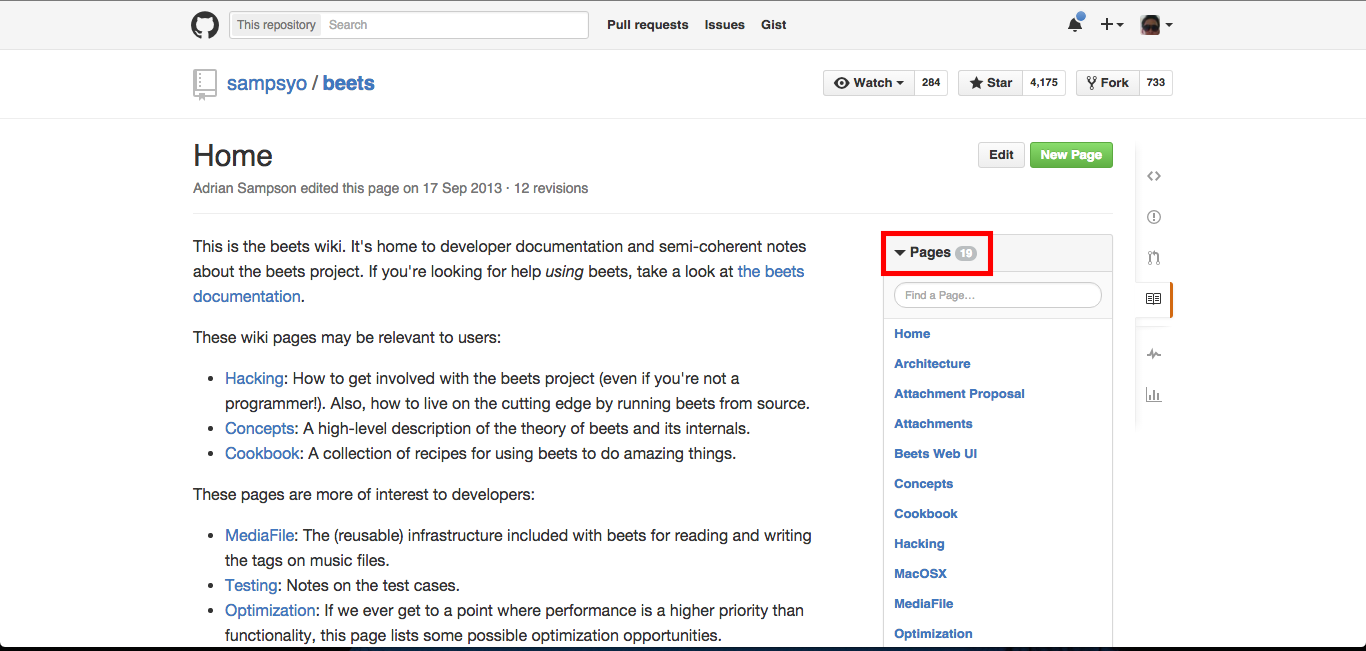
\includegraphics[width=13cm]{Wiki.png}
\caption{Wiki数の調査}\label{tab:Wiki}
\end{figure}

図\ref{tab:Wiki}はWiki数の調査画面である.Pagesの隣の数値がWiki数である.赤枠に囲まれている数値を取得する.所得した数値は,"データ一覧.csv"に保存する.


\subsection{ファイル数,バイト数}

指定のリポジトリをcloneする.
{
\small
\begin{verbatim}
git clone git@github.com:アカウント名/リポジトリ名
\end{verbatim}
}
cloneしたリポジトリの情報を確認する.
右クリックし,「情報をみる」を選択する.
選択すると,バイト数とファイル数が表示される.
表示された数値を,"データ一覧.csv"に保存する.


\subsection{行数}


指定のリポジトリをcloneする.
{
\small
\begin{verbatim}
git clone git@github.com:アカウント名/リポジトリ名
\end{verbatim}
}
cloneしたリポジトリをターミナルで開く.
ターミナルで,以下のコマンドをうつ.
{
\small
\begin{verbatim}
grep -rI '' リポジトリ名 | wc -l
\end{verbatim}
}
行数が出力される.

出力された行数を,"データ一覧.csv"に保存する.

\subsection{日数}

GitHubが提供しているAPIを用いる.

最初のcommitした日をプロジェクト開始日とする.
最後のcommitした日をプロジェクト終了日とする.
これは,すでに終了しているプロジェクトや,commitが長期間されていないプロジェクトを考慮しているためである.

まず.APIを用いて,すべてのcommitを取得する.
{
\small
\begin{verbatim}
python api.py https://api.github.com/repos/ユーザ名/リポジトリ名/commits?per_page=100 > ユーザ名.リポジトリ名.-commits.txt
\end{verbatim}
}
すべてのcommitから最初と最後のcommitを特定し,日付を取得する.
取得した数値を,"データ一覧.csv"に保存する.




\subsection{一日あたりの行数}
一日あたりの行数は,行数をプロジェクト経過日数で割る.
\subsection{1人日あたりの行数}
1人日あたりの行数は,行数をプロジェクト経過日数と人数で割る.

\subsection{一日あたりのcommit数}
一日あたりのcommit数は,commit数をプロジェクト経過日数で割る.
\subsection{1人日あたりのcommit数}
1人日あたりのcommit数は,commit数をプロジェクト経過日数と人数で割る.





\subsection{開発フロー}
開発フローの特徴とプロジェクトの特徴を照らし合わせる.
\subsubsection{GitHubフロー}
master branchから記述的な名前のbranchがある場合は,GitHubフローである.

\begin{figure}[H]
\centering 
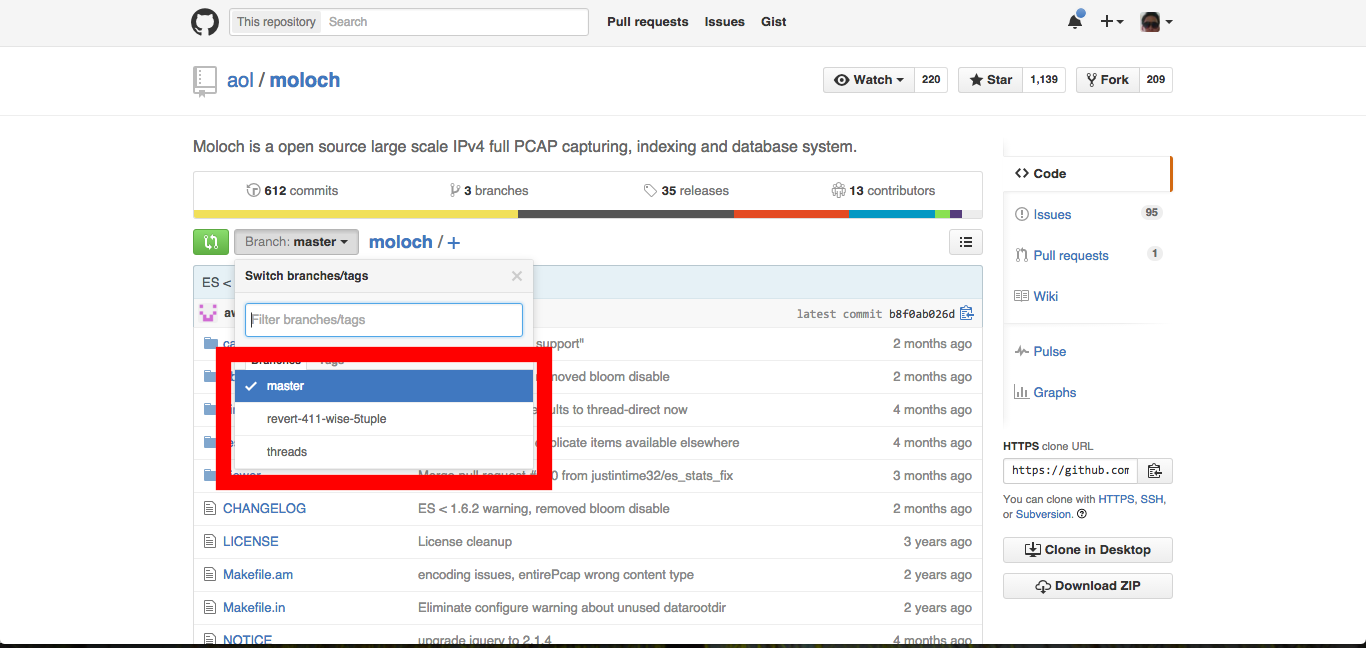
\includegraphics[width=13cm]{githubflow.png}
\caption{GitHubフローの調査}\label{githubフロー}
\end{figure}

\subsubsection{Gitフロー}
develop branchとrelease branchがある場合は,Gitフローである.
\begin{figure}[H]
\centering 
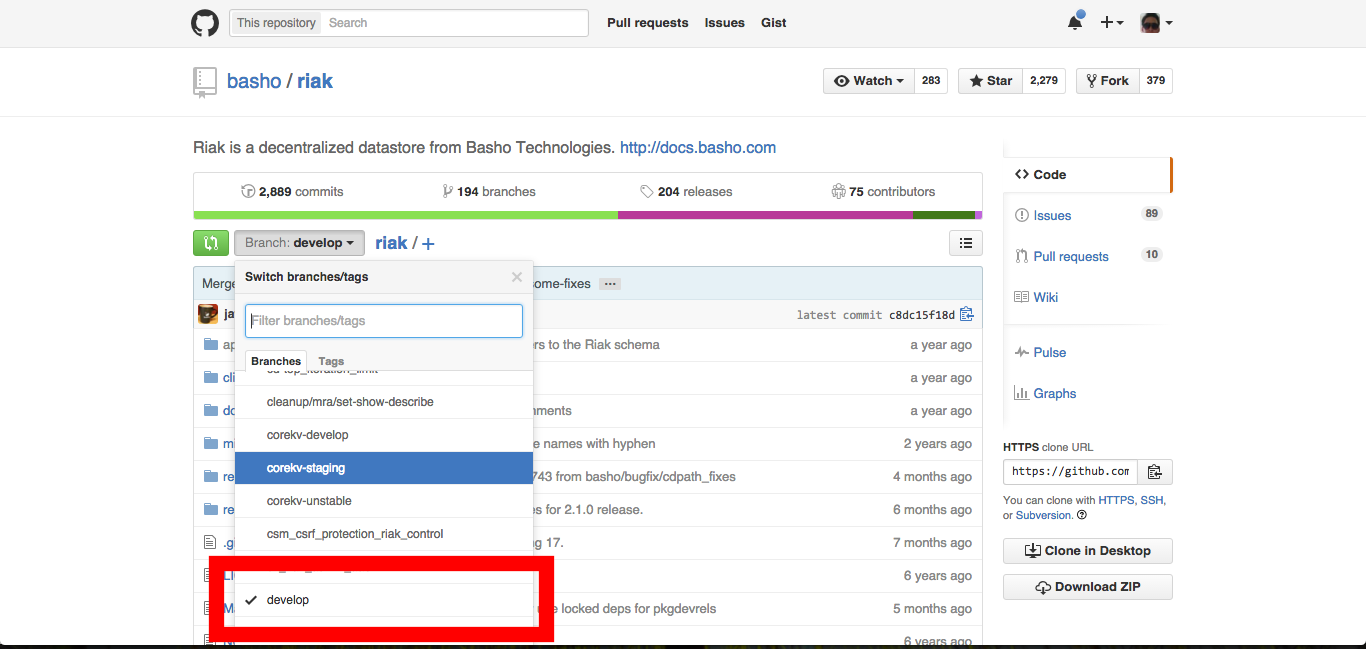
\includegraphics[width=13cm]{gitflow1.png}
\caption{Gitフローの調査}\label{tab:gitフロー1}
\end{figure}
\begin{figure}[H]
\centering 
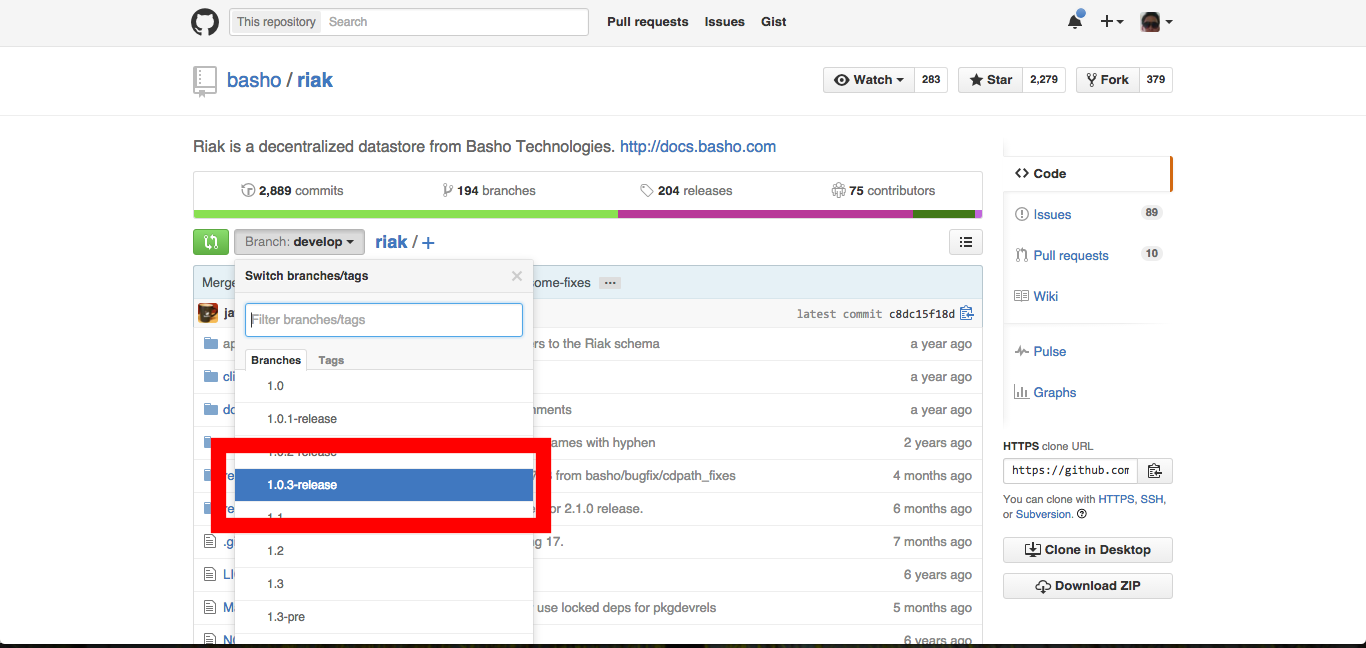
\includegraphics[width=13cm]{gitflow2.png}
\caption{Gitフローの調査}\label{tab:gitフロー2}
\end{figure}

\subsubsection{LINEフロー}
バージョンごとにbranchが作られている場合は,LINEフローである.
\begin{figure}[H]
\centering 
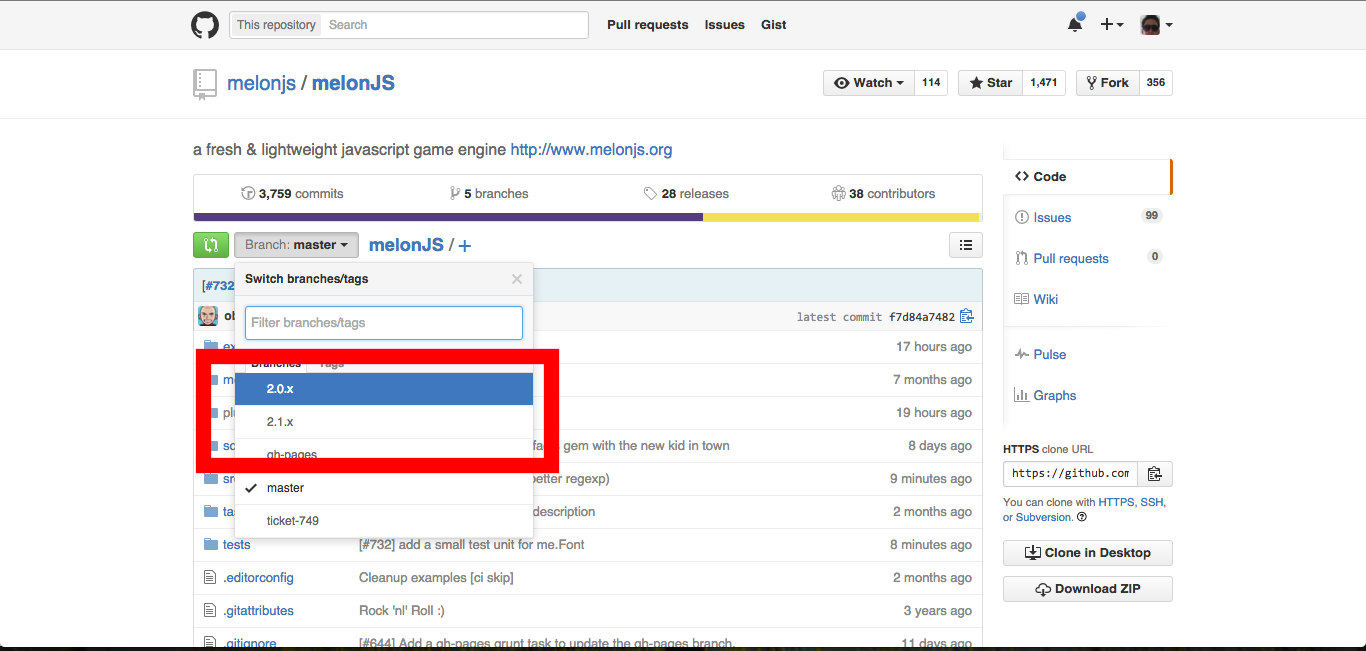
\includegraphics[width=13cm]{lineflow.png}
\caption{LINEフローの調査}\label{tab:lineフロー}
\end{figure}

\subsubsection{日本CAWフロー}
Pull Requestに[WIP]がある場合は,日本CAWフローである.
\begin{figure}[H]
\centering 
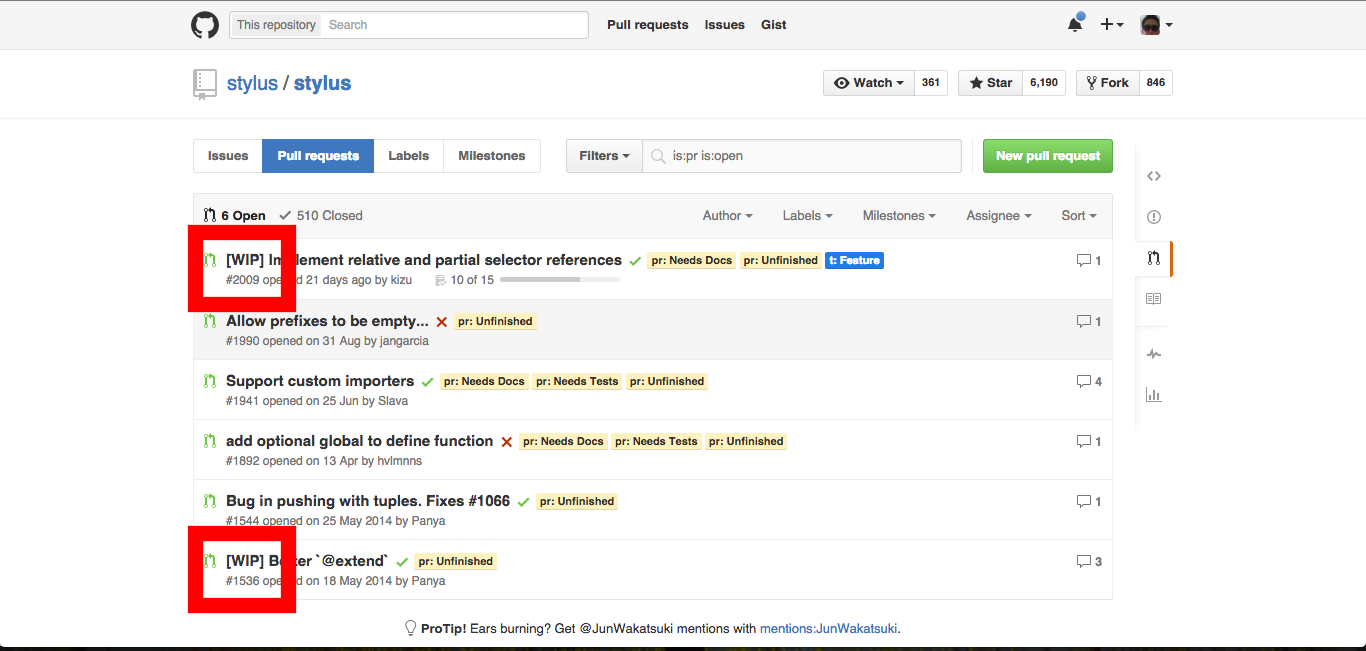
\includegraphics[width=13cm]{wipflow.png}
\caption{日本CAWフローの調査}\label{tab:wipフロー}
\end{figure}


\subsubsection{GitLabフロー}
branchにstableがある場合は,GitLabフローである.
\begin{figure}[H]
\centering 
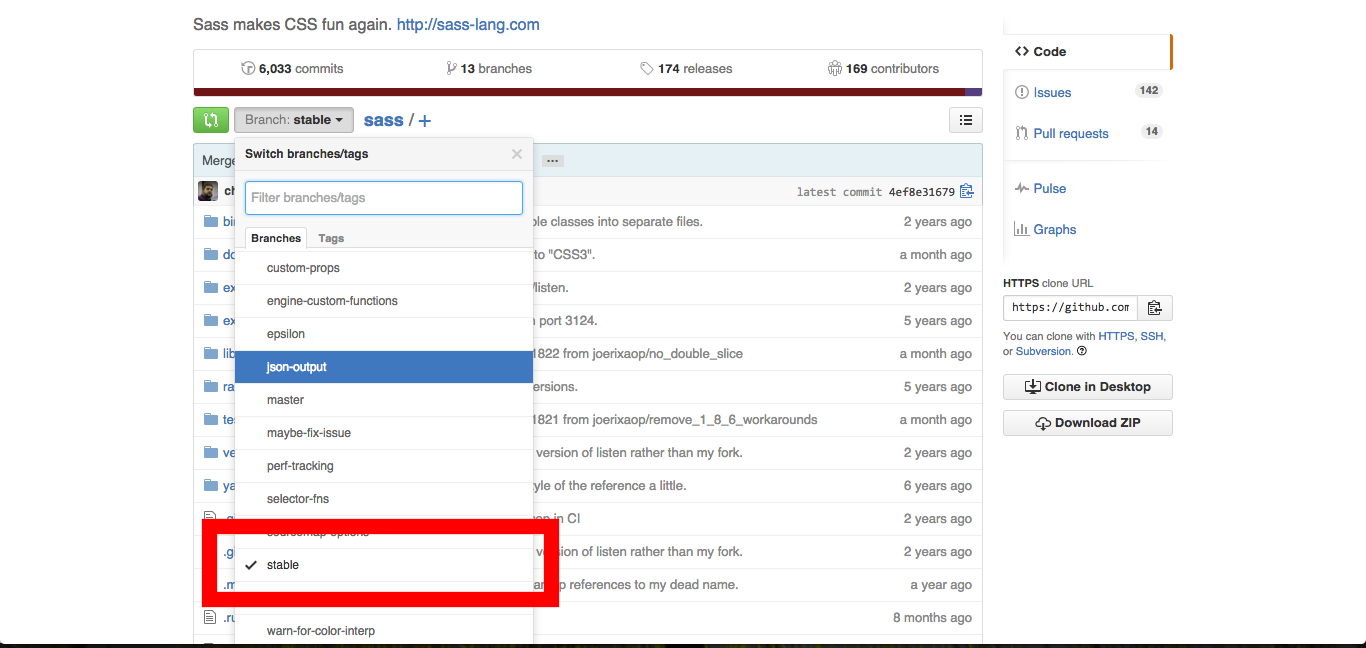
\includegraphics[width=13cm]{GitLabflow.png}
\caption{GitLabフローの調査}\label{tab:GitLabフロー}
\end{figure}


\subsection{コマンドの説明}

調査に用いたコマンドの説明を,以下に記述する.
\subsubsection{requests}
人が使いやすいように設計されていて,Pythonで書かれているApache2 LicensedベースのHTTPライブラリである.
\subsubsection{sudo}
UNIXおよび,UNIX系オペレーティングシステムのプログラムの1つで,ユーザが別のユーザの権限レベルでプログラムを実行するためのコマンドである.
\subsubsection{echo}
文字列を出力するコマンド
\subsubsection{apt-get}
パッケージを取得してインストール/アップデートするDebianプロジェクトが開発したパッケージ管理システムである.
\subsubsection{chmod}
UNIXおよび,UNIX系オペレーティングシステムにおけるシェルコマンドの一種である.ファイルやディレクトリのファイルモードを変更するのに使われる.
\subsubsection{grep}
ファイルの中の文字列を検索する.
\subsubsection{-r}
各ディレクトリ下のすべてのファイルを再帰的に読み取る.
\subsubsection{-I}
バイナリファイルを無視する.
\subsubsection{|}
コマンドの標準出力を次のコマンドに渡す処理を行う.
\subsubsection{wc}
テキスト・ファイルの行数,単語数,バイト数を表示する.
\subsubsection{-l}
行数のみ集計し表示する.



\section{分析ツール}
分析に使うツールは,ExcelとRである.Excelは,集めたデータを分析用のデータに分別したり,保存しておくために使う.Rは,集めたデータを分析するために使う.

Rとは,統計計算をしたり,その結果をグラフにまとめるための言語・環境で,ボランティアによって作られた,S-PLUSの主要な関数をほぼ備えたGNU版(コピーフリー版)です.1991年,ニュージーランド,オークランド大学統計学科の2人の講師,Ross IhakaとRobert Gentlemant によって開発が始まり,現在も開発が進められています\cite{takeuti2005}.


\subsection{Rパッケージのインストール}
決定木分析を,Rで行う方法を記述する.

3種類のパッケージをインストールする
{
\small
\begin{verbatim}
options(repos=c(CRAN="http://cran.ism.ac.jp"))
\end{verbatim}
}

"rattle"をインストールする."rattle"とは,
{
\small
\begin{verbatim}
install.packages("rattle")
\end{verbatim}
}
成功すると以下の画面になる.
\begin{figure}[H]
\centering 
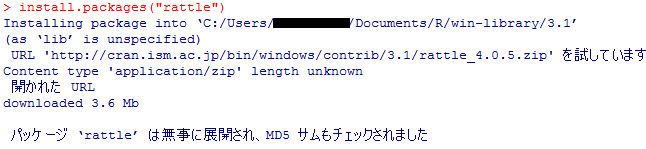
\includegraphics[width=13cm]{rattle.png}
\caption{rattleインストール成功画面}\label{rattle}
\end{figure}

"RColorBrewer"をインストールする."RColorBrewer"とは,様々な美しいカラーパレットが含まれているパッケージである.
{
\small
\begin{verbatim}
install.packages("RColorBrewer")
\end{verbatim}
}
成功すると以下の画面になる.
\begin{figure}[H]
\centering 
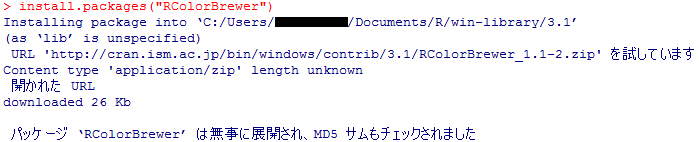
\includegraphics[width=13cm]{RColorBrewer.png}
\caption{RColorBrewerインストール成功画面}\label{RColorBrewer}
\end{figure}

"rpart.plot"をインストールする."rpart.plot"とは,視覚的に表示するためのパッケージである.
{
\small
\begin{verbatim}
install.packages("rpart.plot")
\end{verbatim}
}
成功すると以下の画面になる.
\begin{figure}[H]
\centering 
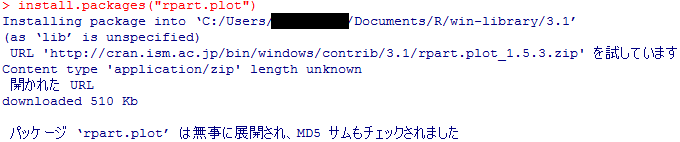
\includegraphics[width=13cm]{rpartPlot.png}
\caption{rpartPlotインストール成功画面}\label{rpartPlot}
\end{figure}


\section{分析データ準備}


\subsection{全てのデータをまとめる}
Excelのcsvファイルに調査した全てのデータを保存する.
実際に保存したデータが図\ref{tab:itiran}である.

\begin{figure}[H]
\centering 
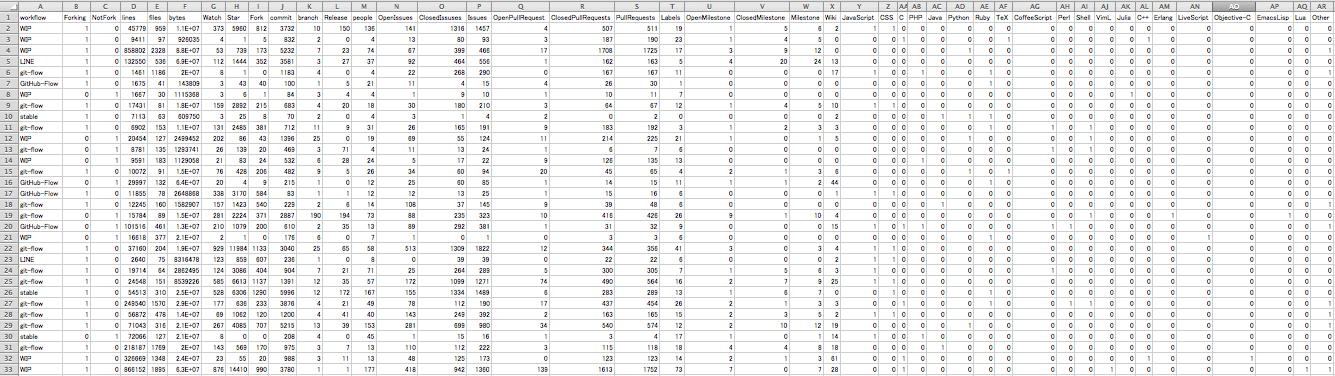
\includegraphics[width=13cm]{allData.png}
\caption{すべてのデータ一覧}\label{tab:itiran}
\end{figure}
Y列からは,言語になっている.
その言語があった場合は1,ない場合は0を入れている.


\subsection{全ての2つにわける}
データをランダムに並び替え,2つにわける.ランダムに分ける方法は,ExcelのRAND関数を使用する.
わけられたデータで,それぞれ決定木分析を行う.

分けられたデータが図\ref{tab:itiran-1}と図\ref{tab:itiran-2}である.
\begin{figure}[H]
\centering 
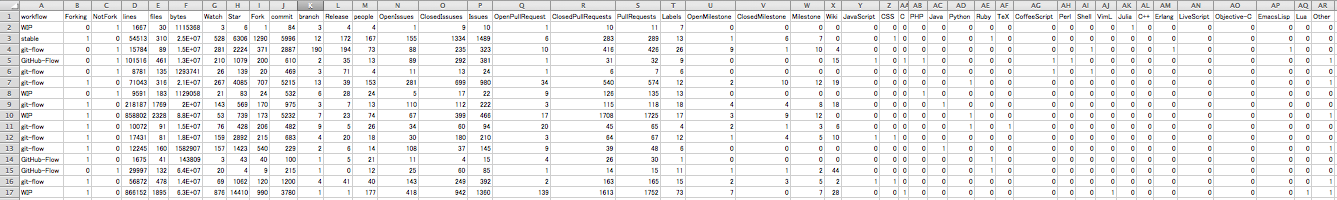
\includegraphics[width=13cm]{allData1.png}
\caption{半分のデータ-1}\label{tab:itiran-1}
\end{figure}
\begin{figure}[H]
\centering 
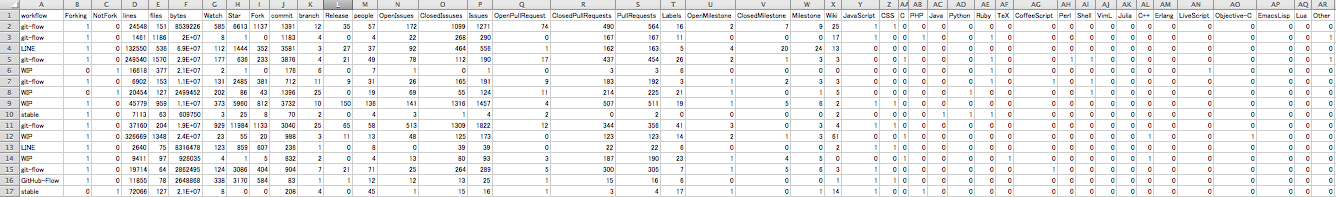
\includegraphics[width=13cm]{allData2.png}
\caption{半分のデータ-2}\label{tab:itiran-2}
\end{figure}


\subsection{コントロールできる要因かつ,成功プロジェクトの場合}

プロジェクトが適切な開発フローを選択していることを実証する.
プロジェクトが成功している場合,適切な開発フローを選択していることにする.
プロジェクトが成功している場合の定義は,リリース数が1以上の時である.

また,選択基準を,プロジェクトが始められる時に使えるように,コントロールできる要因のみにする.
コントロールできる要因とは,行数,プロジェクト経過日数,一日あたりの行数,一人日あたりの行数人数,言語である.

プロジェクトが成功している場合のデータをまとめたデータが図\ref{only}である.


\begin{figure}[H]
\centering 
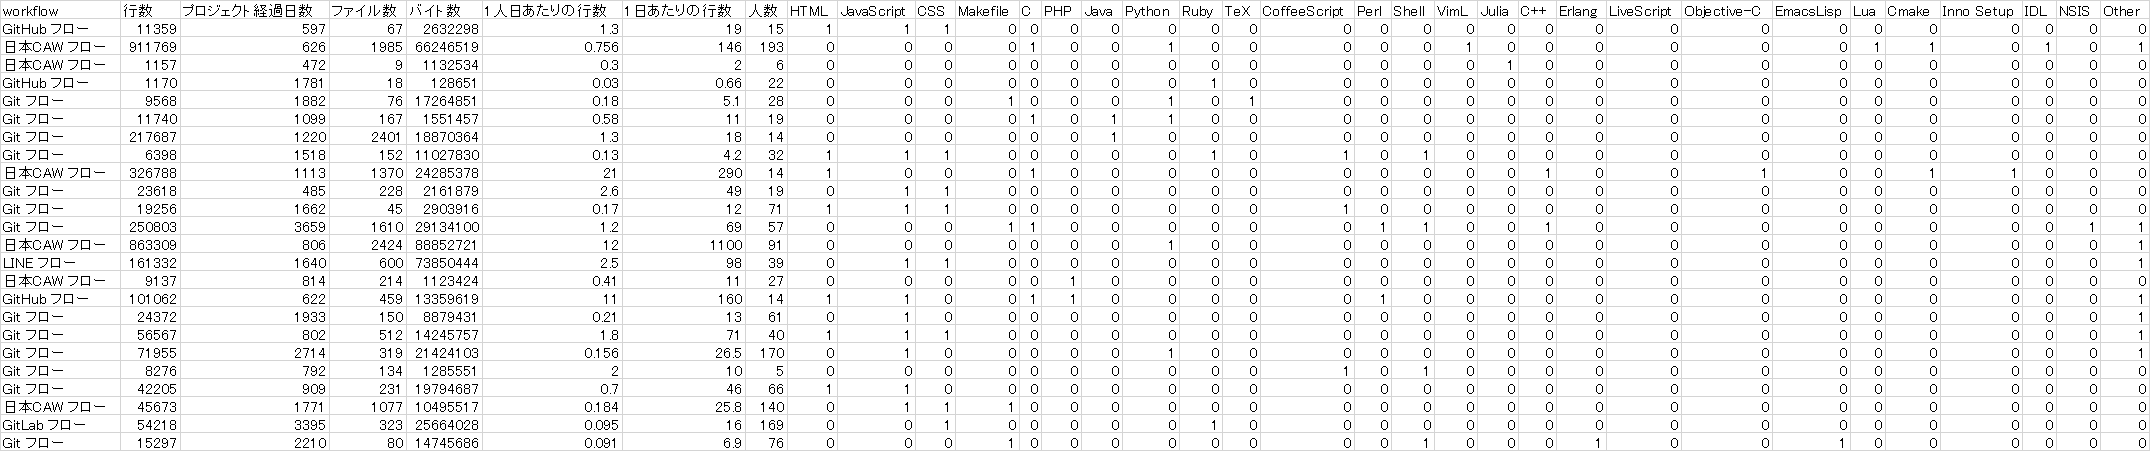
\includegraphics[width=13cm]{onlyData.png}
\caption{コントロールできる要因かつ,成功プロジェクト}\label{only}
\end{figure}



\section{階層的クラスター分析方法}

"データ一覧.csv"のデータを読み込み,データセット"myData"に保存する.
1行目は,行ラベルということにして,データを読み込む.

{
\small
\begin{verbatim}
myData <- read.csv("データ一覧.csv", row.names=1)
\end{verbatim}
}


標準化してから距離を求める.
標準化とは,各列の平均を0,分散を1にすることである.
{
\small
\begin{verbatim}
(myDistanceMatrix <- dist(scale(myData)))
\end{verbatim}
}


階層的クラスター分析を実行する.
{
\small
\begin{verbatim}
myClusters <- hclust(myDistanceMatrix)
\end{verbatim}
}

分析結果を表示する
{
\small
\begin{verbatim}
plot(myClusters, hang = -1)
\end{verbatim}
}





\section{決定木分析方法}

"データ一覧.csv"のデータを読み込み,データセット"myData"に保存する.
{
\small
\begin{verbatim}
myData <- read.csv("データ一覧.csv")
\end{verbatim}
}


データセット"myData"を読み込む.
{
\small
\begin{verbatim}
head(myData)
\end{verbatim}
}

libraryの"mypart"と"maptools"を読み込む
{
\small
\begin{verbatim}
library(mypart)
library(maptools)
\end{verbatim}
}
"myData"のデータをデータセット"myTree"に保存する
{
\small
\begin{verbatim}
myTree <- rpart(workフロー~ .,data = myData)
myTree
\end{verbatim}
}


決定木を描画する.
{
\small
\begin{verbatim}
fancyRpartPlot(myTree)
\end{verbatim}
}
成功すると以下の画面になる.
\begin{figure}[H]
\centering 

\includegraphics[width=13cm]{R.png}
\caption{分析成功画面}\label{R}
\end{figure}






\section{決定木性能測定方法}

決定木性能測定方法を記述する.


\subsection{訓練データとテストデータの準備}
データをランダムに2種類に分ける.一方は,16件の訓練データ,もう一方は,8件のテストデータに分ける.

ランダムに分ける方法は,ExcelのRAND関数を使用する.

16件の訓練データで,决定木を作る.
8件のテストデータで,精度と再現率を求める.


これを10回行い,10通りのデータを用意する.

\subsection{平均と信頼区間を求める}
平均は,ExcelのAVERAGE関数を用いる.
標準偏差は,STDEVP関数を用いる.
信頼区間は,CONFIDENCE関数を用いる.


\chapter{結果}

\section{階層的クラスター分析結果}


2種類のデータを用いて,Rで決定決定木分析を行った.
すべてのデータで行った場合,
コントロールできる要因のみかつ,成功しているプロジェクトの場合である.

次に,それぞれの結果を記述する.
\subsection{すべてのデータで行った場合}
図\ref{allCluster}は,すべてのデータで分析を行った結果である.
\begin{figure}[H]
\centering 
\includegraphics[width=13cm]{allCluster.eps}
\caption{全てのデータで作った場合}\label{allCluster}
\end{figure}

\subsection{コントロールできる要因のみかつ,成功しているプロジェクトの場合}
図\ref{onlyCluster}は図\ref{only}を用いて分析を行った結果である.

\begin{figure}[H]
\centering 
\includegraphics[width=13cm]{onlyCluster.eps}
\caption{コントロールできる要因かつ,成功しているプロジェクトの場合}\label{onlyCluster}
\end{figure}










\section{決定木分析結果}
3種類のデータを用いて,Rで決定決定木分析を行った.
すべてのデータで行った場合,
データをランダムに並び替え,2つに分けた場合,
コントロールできる要因のみかつ,成功しているプロジェクトの場合である.

次に,それぞれの結果を記述する.
\subsection{すべてのデータで行った場合}
図\ref{決定木}は,すべてのデータで分析を行った結果である.
\begin{figure}[H]
\centering 
\includegraphics[width=13cm]{allDecisionTree.eps}
\caption{全てのデータで作った決定木}\label{決定木}
\end{figure}

すべてのデータで分析した場合,Star数,人数,Open Pull Request数,Watch数,ファイル数,branch数,JavaScriptで別れた.


\subsection{データをランダムに並び替え,2つに分けた場合}



図\ref{half決定木1}は,図\ref{tab:itiran-1}を用いて分析を行った結果である.
図\ref{half決定木2}は,図\ref{tab:itiran-2}を用いて分析を行った結果である.




\begin{figure}[H]
\centering 
\includegraphics[width=13cm]{half1.eps}
\caption{決定木-1}\label{half決定木1}
\end{figure}

\begin{figure}[H]
\centering 
\includegraphics[width=13cm]{half2.eps}
\caption{決定木-2}\label{half決定木2}
\end{figure}

データをランダムに2つに分けた場合,異なった結果がでた.
図\ref{half決定木1}は,Issue数,ファイル数で別れた.
図\ref{half決定木2}は,Ruby,行数,バイト数で別れた.

最も重要なファクターが全ての決定木で異なることがわかる.
図\ref{half決定木1}では,Issue数である.
図\ref{half決定木2}では,Rubyである.
また,別の決定木では,これらファクターは出てきていない.




\subsection{コントロールできる要因のみかつ,成功しているプロジェクトの場合}

図\ref{onlyDecision}は図\ref{only}を用いて分析を行った結果である.

\begin{figure}[H]
\centering 
\includegraphics[width=13cm]{onlyDecitionTree.eps}
\caption{コントロールできる要因かつ,成功しているプロジェクトの場合}\label{onlyDecision}
\end{figure}



\section{決定木性能測定結果}
図\ref{onlyDecision}の性能を測定する.
性能を測定した10回分の結果を,次に記す.


\subsection{1回目}
1回目に,決定木分析に使ったデータは,図\ref{データ1-1}である.
図\ref{データ1-1}の決定木分析結果は,図\ref{決定木1}である.
図\ref{決定木1}の性能を測定するのに使ったテストデータは,図\ref{データ1-2}である.

1回目の性能測定の結果,精度は,37.5%だった.再現率は,50.0%だった.
\begin{figure}[H]
\centering 
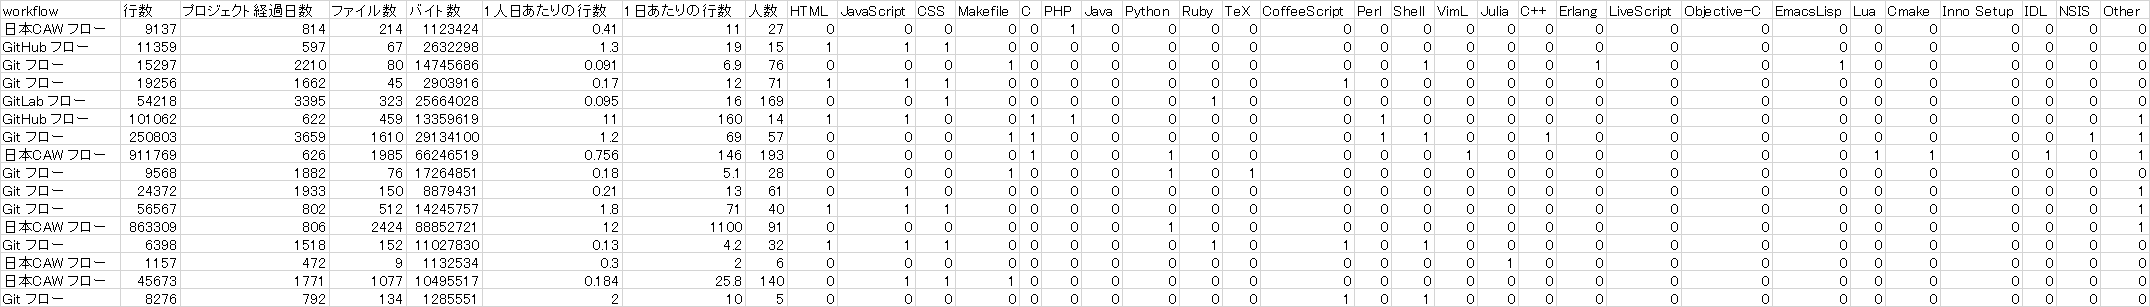
\includegraphics[width=13cm]{1-1.png}
\caption{訓練データ-1}\label{データ1-1}
\end{figure}
\begin{figure}[H]
\centering 
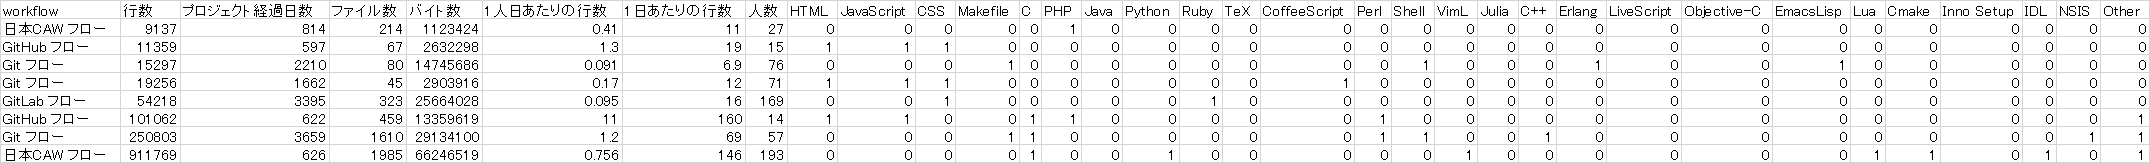
\includegraphics[width=13cm]{1-2.png}
\caption{テストデータ-1}\label{データ1-2}
\end{figure}
\begin{figure}[H]
\centering 
\includegraphics[width=13cm]{1.eps}
\caption{性能測定用決定木-1}\label{決定木1}
\end{figure}

\subsection{2回目}
2回目に,決定木分析に使ったデータは,図\ref{データ2-1}である.
図\ref{データ2-1}の決定木分析結果は,図\ref{決定木2}である.
図\ref{決定木2}の性能を測定するのに使ったテストデータは,図\ref{データ2-2}である.


2回目の性能測定の結果,精度は,50.0%だった.再現率は,57.1%だった.

\begin{figure}[H]
\centering 
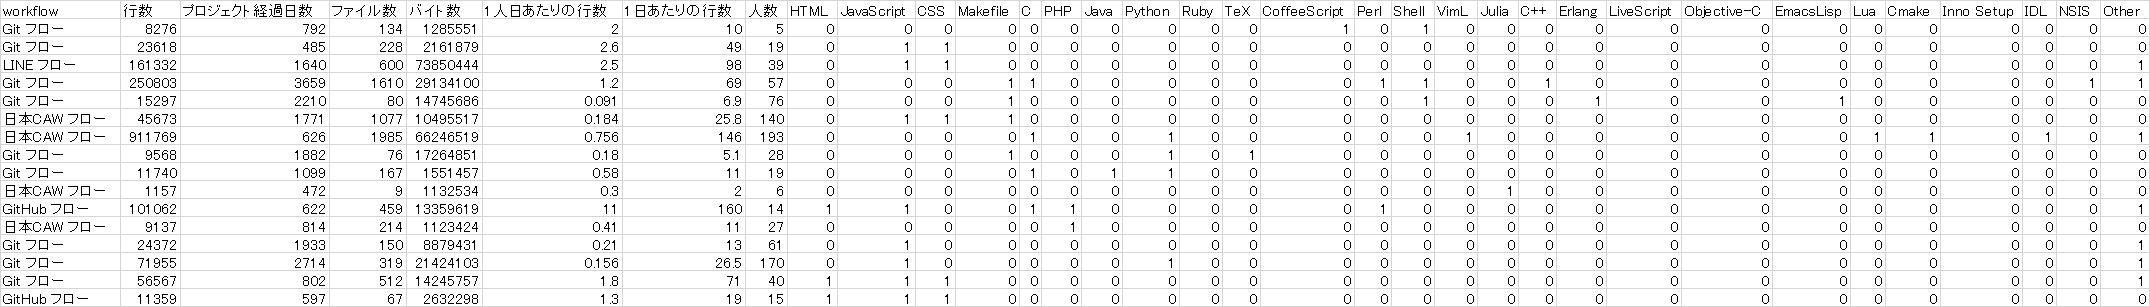
\includegraphics[width=13cm]{2-1.png}
\caption{訓練データ-2}\label{データ2-1}
\end{figure}
\begin{figure}[H]
\centering 
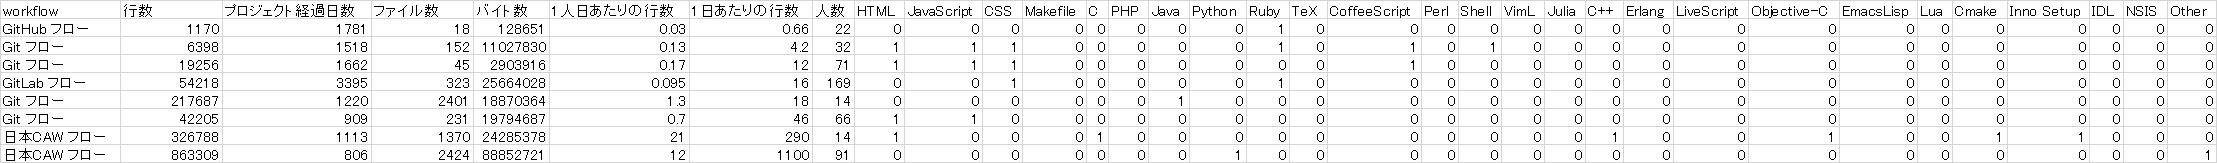
\includegraphics[width=13cm]{2-2.png}
\caption{テストデータ-2}\label{データ2-2}
\end{figure}
\begin{figure}[H]
\centering 
\includegraphics[width=13cm]{2.eps}
\caption{性能測定用決定木-2}\label{決定木2}
\end{figure}


\subsection{3回目}
3回目に,決定木分析に使ったデータは,図\ref{データ3-1}である.
図\ref{データ3-1}の決定木分析結果は,図\ref{決定木3}である.
図\ref{決定木3}の性能を測定するのに使ったテストデータは,図\ref{データ3-2}である.


3回目の性能測定の結果,精度は,37.5%だった.
再現率は,50.0%だった.


\begin{figure}[H]
\centering 
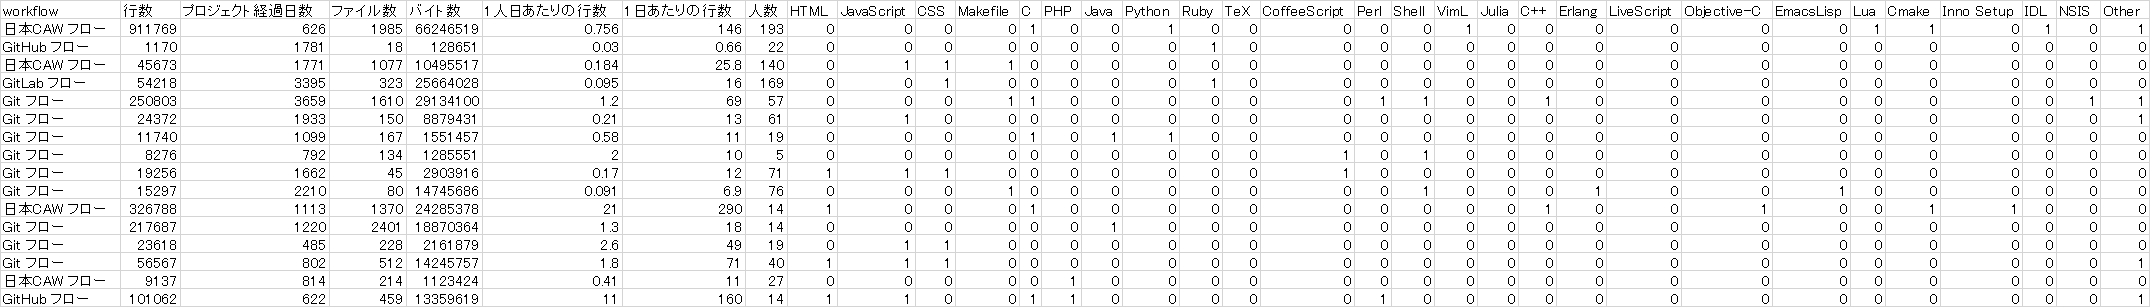
\includegraphics[width=13cm]{3-1.png}
\caption{訓練データ-3}\label{データ3-1}
\end{figure}
\begin{figure}[H]
\centering 
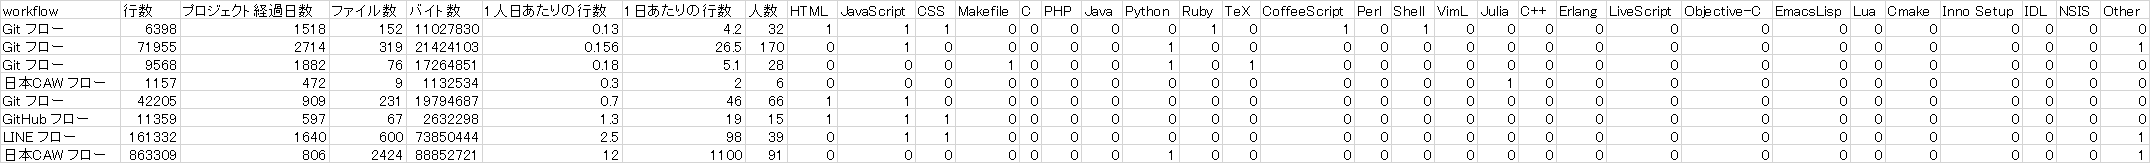
\includegraphics[width=13cm]{3-2.png}
\caption{テストデータ-3}\label{データ3-2}
\end{figure}
\begin{figure}[H]
\centering 
\includegraphics[width=13cm]{3.eps}
\caption{性能測定用決定木-3}\label{決定木3}
\end{figure}


\subsection{4回目}
4回目に,決定木分析に使ったデータは,図\ref{データ4-1}である.
図\ref{データ4-1}の決定木分析結果は,図\ref{決定木4}である.
図\ref{決定木4}の性能を測定するのに使ったテストデータは,図\ref{データ4-2}である.

4回目の性能測定の結果,精度は,37.5%だった.
再現率は,37.5%だった.

\begin{figure}[H]
\centering 
\includegraphics[width=13cm]{4-1.png}
\caption{訓練データ-4}\label{データ4-1}
\end{figure}
\begin{figure}[H]
\centering 
\includegraphics[width=13cm]{4-2.png}
\caption{テストデータ-4}\label{データ4-2}
\end{figure}
\begin{figure}[H]
\centering 
\includegraphics[width=13cm]{4.eps}
\caption{性能測定用決定木-4}\label{決定木4}
\end{figure}


\subsection{5回目}
5回目に,決定木分析に使ったデータは,図\ref{データ5-1}である.
図\ref{データ5-1}の決定木分析結果は,図\ref{決定木5}である.
図\ref{決定木5}の性能を測定するのに使ったテストデータは,図\ref{データ5-2}である.

5回目の性能測定の結果,精度は,37.5%だった.
再現率は,42.9%だった.

\begin{figure}[H]
\centering 
\includegraphics[width=13cm]{5-1.png}
\caption{訓練データ-5}\label{データ5-1}
\end{figure}
\begin{figure}[H]
\centering 
\includegraphics[width=13cm]{5-2.png}
\caption{テストデータ-5}\label{データ5-2}
\end{figure}
\begin{figure}[H]
\centering 
\includegraphics[width=13cm]{5.eps}
\caption{性能測定用決定木-5}\label{決定木5}
\end{figure}


\subsection{6回目}
6回目に,決定木分析に使ったデータは,図\ref{データ6-1}である.
図\ref{データ6-1}の決定木分析結果は,図\ref{決定木6}である.
図\ref{決定木6}の性能を測定するのに使ったテストデータは,図\ref{データ6-2}である.

6回目の性能測定の結果,精精度は,37.5%だった.
再現率は,42.9%だった.

\begin{figure}[H]
\centering 
\includegraphics[width=13cm]{6-1.png}
\caption{訓練データ-6}\label{データ6-1}
\end{figure}
\begin{figure}[H]
\centering 
\includegraphics[width=13cm]{6-2.png}
\caption{テストデータ-6}\label{データ6-2}
\end{figure}
\begin{figure}[H]
\centering 
\includegraphics[width=13cm]{6.eps}
\caption{性能測定用決定木-6}\label{決定木6}
\end{figure}


\subsection{7回目}
7回目に,決定木分析に使ったデータは,図\ref{データ7-1}である.
図\ref{データ7-1}の決定木分析結果は,図\ref{決定木7}である.
図\ref{決定木7}の性能を測定するのに使ったテストデータは,図\ref{データ7-2}である.

7回目の性能測定の結果,精精度は,25.0%だった.
再現率は,50.0%だった.

\begin{figure}[H]
\centering 
\includegraphics[width=13cm]{7-1.png}
\caption{訓練データ-7}\label{データ7-1}
\end{figure}
\begin{figure}[H]
\centering 
\includegraphics[width=13cm]{7-2.png}
\caption{テストデータ-7}\label{データ7-2}
\end{figure}
\begin{figure}[H]
\centering 
\includegraphics[width=13cm]{7.eps}
\caption{性能測定用決定木-7}\label{決定木7}
\end{figure}


\subsection{8回目}
8回目に,決定木分析に使ったデータは,図\ref{データ8-1}である.
図\ref{データ8-1}の決定木分析結果は,図\ref{決定木8}である.
図\ref{決定木8}の性能を測定するのに使ったテストデータは,図\ref{データ8-2}である.

8回目の性能測定の結果,精精度は,37.5%だった.
再現率は,42.9%だった.

\begin{figure}[H]
\centering 
\includegraphics[width=13cm]{8-1.png}
\caption{訓練データ-8}\label{データ8-1}
\end{figure}
\begin{figure}[H]
\centering 
\includegraphics[width=13cm]{8-2.png}
\caption{テストデータ-8}\label{データ8-2}
\end{figure}
\begin{figure}[H]
\centering 
\includegraphics[width=13cm]{8.eps}
\caption{性能測定用決定木-8}\label{決定木8}
\end{figure}


\subsection{9回目}
9回目に,決定木分析に使ったデータは,図\ref{データ9-1}である.
図\ref{データ9-1}の決定木分析結果は,図\ref{決定木9}である.
図\ref{決定木9}の性能を測定するのに使ったテストデータは,図\ref{データ9-2}である.

9回目の性能測定の結果,精精度は,50.0%だった.
再現率は,57.1%だった.

\begin{figure}[H]
\centering 
\includegraphics[width=13cm]{9-1.png}
\caption{訓練データ-9}\label{データ9-1}
\end{figure}
\begin{figure}[H]
\centering 
\includegraphics[width=13cm]{9-2.png}
\caption{テストデータ-9}\label{データ9-2}
\end{figure}
\begin{figure}[H]
\centering 
\includegraphics[width=13cm]{9.eps}
\caption{性能測定用決定木-9}\label{決定木9}
\end{figure}


\subsection{10回目}
10回目に,決定木分析に使ったデータは,図\ref{データ10-1}である.
図\ref{データ10-1}の決定木分析結果は,図\ref{決定木10}である.
図\ref{決定木10}の性能を測定するのに使ったテストデータは,図\ref{データ10-2}である.

10回目の性能測定の結果,精精度は,25.0%だった.
再現率は,28.6%だった.

\begin{figure}[H]
\centering 
\includegraphics[width=13cm]{10-1.png}
\caption{訓練データ-10}\label{データ10-1}
\end{figure}
\begin{figure}[H]
\centering 
\includegraphics[width=13cm]{10-2.png}
\caption{テストデータ-10}\label{データ10-2}
\end{figure}
\begin{figure}[H]
\centering 
\includegraphics[width=13cm]{10.eps}
\caption{性能測定用決定木-10}\label{決定木10}
\end{figure}




\subsection{平均と信頼区間}
精度の平均は,37.5\%であった.
精度の信頼区間は,32.6~42.4\%であった.
再現率の平均は,45.9\%であった.
再現率の信頼区間は,40.7~51.1\%であった.

\chapter{考察}



\section{すべてのデータで行った場合}
図\ref{決定木}を考察する.
図\ref{決定木}は,図\ref{tab:itiran}を用いて分析を行った結果である.

図\ref{決定木}より,Star数,人数,OpenPullRequest数,Watch数,ファイル数,branch数,JavaScriptで開発フローを再現できることがわかった.
また,リーフは,GitフローとGitHubフローとLINEフローと日本CAWフローとGitLabフローである.

それぞれの分岐要因を考察していく.

Star数により,選択するフローが変わっている.ここから,開発に直接かかわる人だけでフローが決まらないことが言える.
これは,開発に関心がある人,注目している人も含めて,フローを選択しなければならないことが,想定される.

人数により,選択するフローが変わっている.変わっているのは,Gitフローと日本CAWフローである.
Gitフローと日本CAWフローの大きな違いは,複雑度である.
人数が84人以上の場合,複雑すぎると開発しづらいことから,より複雑度が低い日本CAWフローを選択していることが,想定される.

1日あたりのcommit数により,選択するフローが変わっている.ここからプロジェクトの生産性により,適正な開発フローが異なることが言える.
3番目に重要な指標となっていることから,ほかの生産性の指標を用いることで,より正確なフローを選択できるようになるだろう.

\section{データをランダムに並び替え,2 つに分けた場合}
図\ref{決定木1}と図\ref{決定木2}を比較して,考察する.
図\ref{決定木1}は,図\ref{tab:itiran-1}を用いて分析を行った結果である.
図\ref{決定木2}は,図\ref{tab:itiran-2}を用いて分析を行った結果である.

図\ref{決定木1}は,一日あたりのcommit数とClosedPullRequest数で,分岐している.
また,リーフは,GitフローとGitHubフローと日本CAWフローである.


図\ref{決定木2}は,Watch数とbranch数と人数で,分岐している.
また,リーフは,GitフローとGitHubフローと日本CAWフローである.

2つの決定木を見比べると,分岐が大きく異なっていることがわかる.

大きく異なっていることから,16件に分けられたデータのばらつきが大きいことがわかる.
ここから,精度と再現率が低い可能性があることがわかる.



そのため,決定木の性能測定を行う必要がある.

以上までの考察を含めて,以下の改善を行う.

1つ目は,指標を絞る.
ばらつきが大きいことがわかったため,指標を絞ることにする.
指標を絞ることで,ばらつきを減らし,精度と再現率を上げられると想定する.

指標は,プロジェクト開始時にわかっているものにした.
プロジェクト開始時にわかっているものは,行数と人数と言語と生産性と規模である.

2つ目は,成功しているプロジェクトに絞る.
成功していないプロジェクトを含めると,最適なフローを選択できていない可能性がある.
そのため,データに矛盾が生じている可能性が考えられる.
データに矛盾があると,決定木がうまく再現できない.

成功しているプロジェクトの基準は,リリースを1以上していることにする.


\section{コントロールできる要因のみかつ,成功しているプロジェクトの場合}
図\ref{onlyDecision}を考察する.
図\ref{onlyDecision}は,図\ref{only}を用いて分析を行った結果である.

図\ref{onlyDecision}は,行数とバイト数と1日あたりの行数で,分岐している.
行数とバイト数は,プロジェクトの規模に関わる.
1日あたりの行数は,プロジェクトの生産性に関わる.

分岐より,プロジェクトの規模と生産性が,重要な指標であることがわかった.

プロジェクトが大きくなるにつれて,管理が難しくなる.その管理を助けるためにフローを変える必要があるのだろう.

プロジェクトの生産性は,作業の多さに関わる.テストが多かったり,難しい開発であれば,生産性は大きく変わる.
プロジェクトが進むスピードに比べて,複雑すぎるフローだと,開発を送らせてしまう.
簡単すぎるフローだと,開発を進ませすぎてしまい,バグが多く入ってしまう可能性が考えられる.



\section{精度と再現率}
精度と再現率は,あまりよくない結果になった.

よくない結果になった要因は,人手で選んだ開発フローが間違えている,プロジェクトの重要な指標を調査できていない等があげられる.

人手で選んだ開発フローが間違えていることの対処は,第三者に判定してもらう方法がある.
一人が選択したより,二人が選択したほうが精度は高くなるだろう.

プロジェクトの重要な指標を調査できていないことの対処は,プロジェクトの生産性に注目する.
現在では,日数で割った指標しか用いていない.ここまでの分析で,プロジェクトの生産性が,要因になることがわかった.
そのため,人数の増減傾向や,特定の曜日に開発が進む等,より詳細なプロジェクトの生産性を表していない.
人数の増減傾向は,人がどのタイミングで増減したのかわかれば,指標として用いることが可能だろう.
また,ソフトウェア開発プロジェクトは,開発が進むにつれて人数の変化がある.
開発段階は人数が増加する.納入段階に近づくにつれて,減少が起こる.
特定な曜日に開発が進み,特定の曜日にテストを行うプロジェクトもある.

より詳細な指標を用いれば,新しい要因を作ることが出来,精度と再現率を上げることができるだろう.







\chapter{結論}
本研究により,開発フローを再現手法を提案した.
GitHub上のプロジェクトから性質と開発フローを調査し,决定木分析を行うことで,再現した.

この再現手法は,精度と再現率が高いとはいえない.
精度は,37.5\%だった.再現率は,45.9\%だった.

しかし,精度と再現率を高めることができれば,開発経験の浅いプロジェクトでも,最適なフローを選択できるようになるだろう.



\bibliographystyle{junsrt}
\bibliography{biblio}%「biblio.bib」というファイルが必要.

\end{document}
